\documentclass{agujournal2019}

\usepackage{cmap}
\usepackage[T2A]{fontenc}
\usepackage[utf8]{inputenc}
\usepackage[english,russian]{babel}
\usepackage{amsmath,amssymb}
\usepackage{graphicx}
\usepackage{siunitx}
\sisetup{output-decimal-marker={,}}
\sisetup{range-phrase=--, range-units=single}
\usepackage{natbib}
\usepackage{hyperref}
\usepackage{booktabs}
\usepackage{array}
\usepackage{tabularx}
\usepackage{lineno}
\setlength{\emergencystretch}{2em}

\journalname{Space Weather}

\renewenvironment{keypoints}{%
  \subsection*{Ключевые пункты}%
  \begin{itemize}
}{%
  \end{itemize}
}

\renewenvironment{abstract}{%
  \begin{center}
  {\bfseries\large Аннотация}
  \end{center}
  \vspace{-0.5em}
  \small
}{%
  \normalsize
}

\begin{document}

\title{Зависящий от масштаба отклик WSPR на геомагнитные бури: \\
	частотная зависимость и поисковая оценка межпериодного масштабирования абсолютных снижений \\
	\small Scale-dependent WSPR response to geomagnetic storms: \\
	frequency dependence and exploratory period-to-period scaling of absolute loss}

\authors{Alexey Petrov\affil{1}, Makar Petrov\affil{1}}

\affiliation{1}{Независимые исследователи (без аффилиации), Россия}

\linenumbers
\maketitle
\begin{keypoints}
	\item На тренировочном периоде число WSPR-спотов падает на
	\SIrange{27}{39}{\percent} во время бурь с $Kp \ge 5$ на всех трёх
	HF-диапазонах (блочная перестановка, $p \le 2 \times 10^{-5}$);
	скорректированные на ковариаты падения составляют
	\SIrange{27}{40}{\percent}. На отложенном периоде скорректированные
	падения составляют \SIrange{19}{23}{\percent}
	\item Отклик демонстрирует масштабно-зависимую картину: при Kp 5--6
	$\sim$\SI{-18}{\percent}, при Kp $\ge$ 6 $\sim$\SI{-43}{\percent}
	(20/40\,m; 15\,m: от \SI{-28.6}{\percent} до \SI{-54.8}{\percent}).
	Наблюдается монотонный градиент; тест тренда значим для 20\,m и
	15\,m, но маргинален для 40\,m на уровне эпизодов ($p = 0.064$).
	Бины с наибольшим Kp разрежены, и не все сравнения соседних бинов
	разрешены. Первичный эффект воспроизводится по направлению на всех
	трёх диапазонах на отложенном (held-out) периоде (тест остатков
	$p \le 2 \times 10^{-4}$; 95\% CI для исходных значений на 15\,m
	включает ноль)
	\item Абсолютное снижение спотов на 40\,m имеет отношение 1,44; это
	точечная оценка, превышающая ожидаемое масштабирование
	($\approx$1,35), но широкий 95\% CI [0,65, 2,33] совместим как с
	пропорциональным ростом, так и с инвариантностью; процентные падения
	остаются более устойчивой метрикой
\end{keypoints}

\begin{abstract}
	Мы проверяем гипотезу о том, что геомагнитные бури ($Kp \ge 5$) подавляют
	число WSPR-спотов на любительских HF-диапазонах. Используя открытые данные
	wspr.live (почасовое агрегирование, 3 диапазона: 20\,m, 40\,m, 15\,m)
	и индекс $Kp$ GFZ Potsdam, охватывающие 18 месяцев (апрель 2024 --
	сентябрь 2025; 39\,456 WSPR-часов по трём диапазонам, 198 штормовых
	эпох при $Kp \ge 5$), мы находим значимое вызванное бурями снижение
	числа спотов на всех трёх диапазонах: 20\,m: \SI{-27.7}{\percent},
	40\,m: \SI{-27.2}{\percent}, 15\,m: \SI{-38.7}{\percent} (блочная
	перестановка $p \le 2 \times 10^{-5}$ для всех,
	\num{50000} итераций, блок = 24 эпохи = 72\,h). Поскольку штормовые
	эпохи распределены по месяцам и UTC-часам неравномерно, мы также
	оцениваем скорректированные на ковариаты падения на тренировочном
	периоде с помощью модели
	с отрицательным биномиальным распределением (фиксированные эффекты
	месяца, UTC-часа и дня недели, ошибки, кластеризованные по эпизодам):
	20\,m \SI{-33.6}{\percent} (95\% CI
	[\SI{-39.9}{\percent}, \SI{-26.7}{\percent}]), 40\,m
	\SI{-27.1}{\percent} ([\SI{-33.2}{\percent}, \SI{-20.5}{\percent}]), и
	15\,m \SI{-39.8}{\percent} ([\SI{-46.8}{\percent}, \SI{-31.8}{\percent}]).
	Следовательно, исходные значения консервативны для 20\,m и практически
	не меняются для 40\,m.

	Мы наблюдаем масштабно-зависимую картину: падение возрастает от
	$Kp = 5\text{--}6$ ($\sim\SI{-18}{\percent}$) до $Kp \ge 6$
	($\sim\SI{-43}{\percent}$) на 20/40\,m (15\,m: от \SI{-28.6}{\percent}
	до \SI{-54.8}{\percent}), что согласуется с нелинейным откликом ионосферы
	на геомагнитное воздействие. Тест тренда на основе блочной перестановки
	значим на всех трёх диапазонах ($p \le 0.02$), однако бины с наибольшим
	$Kp$ разрежены (38 эпох из 12 эпизодов). Наблюдается монотонный
	градиент; тест тренда значим для 20\,m и 15\,m, но маргинален для
	40\,m на уровне эпизодов ($p = 0.064$), поэтому градиент не
	разрешается при наибольшем $Kp$. Первичный эффект воспроизводится по
	направлению на независимом отложенном (held-out) периоде (январь--март
	2026, обновлённая выгрузка из живой базы данных) на всех трёх диапазонах,
	включая 15\,m (блочная перестановка остатков
	$p \le 2 \times 10^{-4}$; его исходный 95\% CI включает ноль). На
	отложенном периоде скорректированные на ковариаты падения составляют
	\SIrange{19}{23}{\percent}, меньше тренировочных значений, но по-прежнему
	исключают ноль.

	Частотная зависимость и поисковый анализ UT-окон
	согласуются с интерпретацией двух механизмов: падение на 15\,m
	(\SI{-38.7}{\percent}) совместимо со снижением MUF, тогда как поглощение
	в слое D влияет на 20\,m/40\,m
	(\SI{-27.7}{\percent}/\SI{-27.2}{\percent}). Асимметрия UT-окон (падение
	на 40\,m сильнее в окне 0--6 UTC в течение 8 месяцев с достаточными
	данными) согласуется с перемежающимся авроральным поглощением и
	поглощением в полярной шапке. Однако агрегированные счётчики спотов
	не позволяют однозначно разделить эти механизмы; среднее SNR
	декодированных спотов меняется во время бурь менее чем на
	\SI{0.5}{dB}, поэтому снижение счёта обусловлено главным образом
	потерей маргинальных декодируемых трасс, а не равномерным уменьшением
	SNR.

	Абсолютное снижение спотов на 40\,m за тренировочный период
	($\SI{-18285}{spots/h}$) первоначально совпадало с held-out-снимком
	($\SI{-18304}{spots/h}$), но повторно скачанная held-out-выборка
	(октябрь 2026) даёт большее абсолютное снижение
	($\SI{-26287}{spots/h}$; отношение 1,44; это точечная оценка,
	превышающая ожидаемое масштабирование ($\approx$1,35), но широкий
	95\% CI [0,65, 2,33] совместим как с пропорциональным ростом, так и с
	инвариантностью). Процентные падения остаются более устойчивой
	метрикой. Все значения абсолютного снижения на held-out основаны на
	обновлённой выгрузке. Эти результаты позволяют
	предположить, что WSPR может служить распределённым ионосферным
	сенсором для обнаружения и характеристики масштабно-зависимых эффектов
	геомагнитных бурь на HF-распространение.
\end{abstract}

\section*{Краткое изложение для широкой аудитории}

Геомагнитные бури возмущают ионосферу — слой атмосферы, который отражает
высокочастотные радиоволны обратно к Земле. Мы проверили, может ли глобальная
сеть любительских радиомаяков (WSPR) обнаруживать эти возмущения. Проанализировав
18 месяцев данных на трёх диапазонах (20\,m, 40\,m, 15\,m), мы обнаружили,
что во время бурь от умеренных до сильных число успешно зарегистрированных
сигналов падает на 27--39 процентов, причём снижение растёт с интенсивностью
бури. Эта картина повторяется в независимом трёхмесячном периоде. Более
сильные эффекты на самом высоком диапазоне согласуются с вызванным бурей
снижением максимальной применимой частоты, тогда как эффект в окне 0--6 UTC
на самом низком диапазоне согласуется с поглощением, вызванным частицами.
Поскольку сеть продолжает расти, абсолютное число потерянных сигналов может
расти вместе с сетью, но текущая неопределённость велика; процентные падения
остаются более устойчивой метрикой мониторинга. Таким образом, данные
радиолюбителей могут служить недорогим, глобально распределённым сенсором
эффектов космической погоды на радиораспространение.


%=============================================================
\section{Введение}
%=============================================================

Распространение высокочастотных (HF) радиоволн в диапазоне
\SIrange{3}{30}{MHz} опирается на ионосферное отражение от слоя F,
критическая частота которого $f_oF_2$ определяет максимальную применимую
частоту (MUF) для данной трассы и угла места \citep{davies1990}. Во время
геомагнитных бурь усиленная магнитосферная конвекция и высыпание частиц
переносят энергию в систему ионосфера--термосфера
\citep{gonzalez1994,tsurutani2003}. Джоулев нагрев повышает температуру
нейтральной атмосферы, вызывая изменения состава, которые увеличивают
относительное содержание молекулярных компонентов (N$_2$, O$_2$) по
сравнению с атомарным кислородом, что, в свою очередь, повышает скорость
рекомбинации в слое F2 \citep{proelss1995}. Итоговый эффект — снижение
$f_oF_2$ и соответствующее понижение MUF, что потенциально нарушает работу
HF-каналов связи, работающих вблизи своей предельной частоты.

Второй, самостоятельный механизм действует на меньших высотах. Высыпание энергичных
частиц (электроны \SIrange{10}{300}{keV} и протоны \SIrange{1}{30}{MeV})
проникает в слой D (\SIrange{60}{90}{km}), повышая электронную концентрацию
и вызывая недевиационное поглощение HF-сигналов
\citep{hargreaves1969,reid1974}. Поскольку поглощение масштабируется как
$\propto 1/f^2$, более низкие HF-диапазоны страдают непропорционально
сильно. Во время бурь это авроральное поглощение и поглощение в полярной
шапке (PCA) может сохраняться часами и распространяться за пределы
аврорального овала.

Weak Signal Propagation Reporter (WSPR) — всемирная сеть любительских
радиомаяков и приёмников, которые автономно обмениваются маломощными
(\SI{<1}{W}--\SI{5}{W}) сигналами на выделенных HF-диапазонах и сообщают
декодированные отношения сигнал/шум в центральную базу данных
\citep{taylor2010}. При тысячах станций, работающих непрерывно, результирующий
набор данных представляет собой распределённый многочастотный ионозонд,
охватывающий географические регионы и трассы распространения за пределами
досягаемости профессиональных сетей зондирования
\citep{frissell2016,labelle2023}.

Предыдущие исследования продемонстрировали полезность данных WSPR для
дистанционного зондирования ионосферы. \citet{frissell2016} показали
качественную связь между картинами WSPR-спотов и геомагнитным возмущением
и предложили WSPR в качестве распределённого ионосферного сенсора в рамках
HamSCI — направления, которое сейчас поддерживается растущим числом
гражданских научных исследований ионосферы
\citep{hamsci2023,cerwin2026,potter2026}. \citet{labelle2023}
проанализировали статистику и покрытие сети WSPR, подтвердив достаточный
трафик для климатологии HF-распространения. \citet{themens2021}
смоделировали авроральный слой D во время бурь с помощью моделей первых
принципов. Независимо \citet{kavanagh2004} представили статистические
наблюдения поведения аврорального слоя D по данным риометров, а
\citet{rodger2010} исследовали влияние высыпания магнитосферных электронов
на среднюю атмосферу.

Несмотря на этот объём работ, количественная многодиапазонная характеристика
отклика WSPR на геомагнитные бури за длительный период отсутствовала.
Существующие исследования WSPR—бурь либо качественные, либо однодиапазонные,
либо охватывают слишком короткие периоды для установления статистической
устойчивости. Насколько нам известно, немногие предыдущие работы сочетали
(i) масштабирование отклика WSPR с интенсивностью бури, (ii) его частотную
зависимость на нескольких одновременно наблюдаемых диапазонах и (iii)
количественную проверку того, остаётся ли абсолютная величина потерь
распространения стабильной при изменении размера сети.

В этой статье мы восполняем эти пробелы пятью вкладами:

\begin{enumerate}
	\item Анализ плотности WSPR-спотов за 18 месяцев на трёх диапазонах
	      (20\,m, 40\,m, 15\,m) во время геомагнитных бурь с использованием
	      индексов $Kp$ и $Dst$ в качестве независимых индикаторов бурь;
	\item Количественная характеристика масштабно-зависимого эффекта:
	      снижение числа спотов растёт с $Kp$, от
	      $\sim\SI{-18}{\percent}$ при $Kp = 5\text{--}6$ до
	      $\sim\SI{-53}{\percent}$ при $Kp \ge 7$;
	\item Независимое воспроизведение на трёхмесячном отложенном
	      (held-out) периоде (январь--март 2026), проверяющее первичный
	      эффект на всех трёх диапазонах;
	\item Проверка масштабирования абсолютного снижения при росте сети:
	      обновлённая held-out-выгрузка даёт отношение абсолютных
	      снижений на 40\,m, равное 1,44; это точечная оценка,
	      превышающая ожидаемое масштабирование ($\approx$1,35) из роста
	      спокойного базового уровня на $\SI{+35}{\percent}$, но широкий
	      95\% CI [0,65, 2,33] совместим как с пропорциональным ростом,
	      так и с инвариантностью, поэтому мы рассматриваем абсолютное
	      снижение как совместимое с масштабированием, связанным с сетью,
	      но не установленное окончательно, тогда как процентные падения
	      остаются более устойчивой метрикой;
	\item Асимметрия UT-окон, согласующаяся с перемежающимся авроральным
	      поглощением и поглощением в полярной шапке во время бурь.
\end{enumerate}


%=============================================================
\section{Данные}
%=============================================================

Источники данных и периоды анализа сведены в таблице~\ref{tab:data};
даты загрузки и статус заморозки перечислены в таблице~\ref{tab:provenance}.

\begin{table}[h]
	\centering
	\caption{Источники данных и покрытие.\protect\footnotemark{}}
	\label{tab:data}
	\begin{tabularx}{\textwidth}{@{}l >{\raggedright\arraybackslash}X >{\raggedright\arraybackslash}X >{\raggedright\arraybackslash}X r@{}}
		\toprule
		Источник               & Переменная                & Разрешение        & Период               & Всего записей \\
		\midrule
		wspr.live (ClickHouse) & WSPR-споты, 3 диапазона   & 1\,h (агрегировано)
		                       & апр. 2024 -- сент. 2025   & 39\,456                                                  \\
		                       &                           &                   & янв. 2026 -- март 2026 (живая база) & 2\,160  \\
		GFZ Potsdam            & индекс $Kp$               & 3\,h
		                       & апр. 2024 -- март 2026    & 5\,069                                                   \\
		WDC Kyoto & индекс $Dst$ (предварительный) & 1\,h
		& апр. 2024 -- сент. 2025 & 12\,508 \\
		\bottomrule
	\end{tabularx}
\end{table}
\footnotetext{Архивный снимок октября 2026 г. содержал $\sim$5\,850 исходных почасовых записей по трём диапазонам; живая повторная выгрузка от 2026-10-15, использованная в этой статье, даёт 720 согласованных 3-часовых эпох на диапазон (всего 2\,160, $N_{\text{storm}} = 47$ на диапазон).}


\begin{table}[h]
	\centering
	\small
	\setlength{\tabcolsep}{4pt}
	\caption{Происхождение данных. Входные данные тренировочного периода
		заморожены; отложенный (held-out) период обслуживается живой базой
		\texttt{wspr.live} (см. раздел~5.5).}
	\label{tab:provenance}
	\begin{tabularx}{\textwidth}{@{}l >{\raggedright\arraybackslash}X >{\raggedright\arraybackslash}X >{\raggedright\arraybackslash}X@{}}
		\toprule
		Набор данных & Содержание & Получено & Хранение / статус заморозки \\
		\midrule
		WSPR-споты (тренировка) & Почасовые агрегаты, 20\,m/40\,m/15\,m,
		апр. 2024 -- сент. 2025 & 7--8 окт. 2026 (wspr.live ClickHouse) &
		\texttt{unified.parquet}; заморожен \\
		индекс $Kp$ & GFZ Potsdam, 3-часовой, апр. 2024 -- март 2026 &
		7--8 окт. 2026 & unified parquet; заморожен \\
		индекс $Dst$ & WDC Kyoto, предварительный, почасовой,
		апр. 2024 -- сент. 2025 & 7--8 окт. 2026 & unified parquet; заморожен \\
		WSPR held-out & Почасовые агрегаты, янв. -- март 2026 &
		8 окт. 2026 (архивный снимок); 15 окт. 2026 (живая
		повторная выгрузка, представлена здесь) & Замороженные parquet-экстракты
		по диапазонам в \texttt{results/} (контрольные суммы sha256
		в манифесте происхождения) \\
		\bottomrule
	\end{tabularx}
\end{table}

\subsection{Сеть WSPR}

Данные WSPR-спотов были получены из зеркала wspr.live ClickHouse с помощью
SQL-запросов: \texttt{SELECT toStartOfHour(time), count(), avg(snr)} из
таблицы \texttt{wspr.rx}, отфильтрованных по индексу диапазона: 14 (20\,m,
\SI{14.0956}{MHz}), 7 (40\,m, \SI{7.0401}{MHz}) и 21 (15\,m,
\SI{21.0961}{MHz}). Почасовое агрегирование снижает требования к хранению
примерно в 100 раз по сравнению с отдельными записями спотов и достаточно
для анализа в масштабе бурь ($\Delta t = 1$\,h при типичной длительности
бури несколько часов). В статье «плотность спотов» — сокращение для этого
почасового агрегированного числа спотов (споты в час на диапазон); она
не нормируется на трассу, станцию или единицу площади.

Тренировочный период охватывает 1 апреля 2024 г. -- 30 сентября 2025 г.
(548 дней, 18 месяцев), что даёт 13\,152 WSPR-часа на диапазон
(39\,456 по трём диапазонам). 18-месячное окно анализа определяется
доступностью полных почасовых данных WSPR по всем трём диапазонам из
зеркала wspr.live ClickHouse; границы не выбирались априори, и никакие
данные не отбрасывались для достижения целевой длины периода. Мы объединяем
почасовые счётчики WSPR с исходным 3-часовым рядом $Kp$ внутренним
соединением (inner join) по точным меткам времени эпох $Kp$, без заполнения
вперёд (forward-filling): каждая эпоха анализа несёт единственный почасовой
счётчик WSPR на метке времени $Kp$ (без 3-часового усреднения), а ряд имеет
3-часовую каденцию. Это даёт 4\,349 согласованных эпох на диапазон
($\approx$13\,047\,h покрытия), из которых 198 эпох удовлетворяют
$Kp \ge 5$ (порог бури, эквивалентный 594\,h). Базовый уровень в спокойное
время ($Kp < 3$) включает 3\,035 эпох и имеет средние числа спотов 73\,718
(20\,m), 67\,105 (40\,m) и 13\,386 спотов/ч (15\,m).

Отложенный (replication) период охватывает январь--март 2026 г. (90 дней).
После того же 3-часового объединения он даёт 47 штормовых эпох на диапазон
(= 141\,h). Это окно немного богаче бурями, чем тренировочное
(47/720 = 6,5\% против 198/4349 = 4,6\% эпох), что важно для интерпретации
отношения абсолютных снижений в разделе~4.6. Оно также имеет более высокий
спокойный базовый уровень из-за роста сети WSPR: 84\,096 спотов/ч
(20\,m, $\SI{+14}{\percent}$), 90\,653 (40\,m, $\SI{+35}{\percent}$)
и 16\,393 (15\,m, $\SI{+22}{\percent}$).

Трёхмесячный разрыв между двумя периодами (октябрь--декабрь 2025 г.)
не используется ни в тренировочном, ни в отложенном анализе, что
обеспечивает строгое временное разделение двух наборов данных.

\subsection{Геомагнитные индексы}

Индекс $Kp$ получен из JSON API GFZ Potsdam в реальном времени
(https://kp.gfz-potsdam.de). $Kp$ — 3-часовой планетарный индекс по
квазилогарифмической шкале от 0 до 9, вычисляемый по данным 13
субавроральных магнитометрических станций. Средний $Kp$ за тренировочный
период составляет 2,29, максимум — 9,0 (несколько событий при 8,7 и выше).
За 18 месяцев 198 3-часовых эпох $Kp$ достигают $Kp \ge 5$ (= 594 штормовых
часа), распределённых по 76 штормовым дням. Сгруппированные в эпизоды,
разделённые более чем 12~h (\texttt{scripts/storm\_episodes.py}), эти эпохи
образуют 58 штормовых эпизодов, поэтому эффективное число независимых
событий существенно меньше числа эпох, и они охватывают все четыре сезона.

Индекс $Dst$ (Disturbance Storm Time) получен из предварительной конечной
точки WDC Kyoto. $Dst$ — почасовой экваториальный индекс кольцевого тока,
вычисляемый по данным четырёх низкоширотных магнитометрических станций.
Он обеспечивает более высокое временное разрешение, чем $Kp$ (почасовое
против 3-часового), и служит независимым индикатором бурь. Предварительные
данные охватывают все 18 месяцев тренировочного периода (средний
$Dst = \SI{-11.5}{nT}$, минимум $Dst = \SI{-96}{nT}$). Всего 471 час
удовлетворяет $Dst < \SI{-50}{nT}$. Эта выборка охватывает меньше штормовых
часов, чем выборка по $Kp$ (471 против 594 часов, т.е.\ 198 трёхчасовых
эпох), но даёт большую согласованную выборку при более высоком почасовом
разрешении (12\,508 почасовых значений против 4\,349 трёхчасовых эпох).

Солнечный радиопоток F10.7 (NOAA SWPC) рассматривался как ковариата, но
через API SWPC доступны только среднемесячные значения, что слишком грубо
для почасового анализа. Существует конечная точка суточного/почасового
F10.7 (SWPC \texttt{f107\_cm\_flux.json}), но она охватывает только
скользящее окно $\sim$40 дней; историческая суточная запись за тренировочный
период (апрель 2024 -- сентябрь 2025) требует архива NGDC Penticton,
который был недоступен для этого анализа.


%=============================================================
\section{Методы}
%=============================================================

\subsection{Суточно-сезонные остатки}

Плотность WSPR-спотов демонстрирует сильный суточный цикл с вариацией
$\sim$2--6$\times$ по диапазонам и UTC-часам
(рисунок~\ref{fig:timeseries}) и систематические межмесячные различия
базового уровня из-за сезонных изменений ионосферных условий и активности
станций. Чтобы изолировать геомагнитный эффект от этих мешающих факторов,
мы вычисляем остатки:

\begin{equation}
	\text{baseline} = \operatorname{mean}(\text{spots} \mid \text{month},
	\text{hour\_of\_day}, \text{day\_of\_week})
	\label{eq:baseline}
\end{equation}

\begin{equation}
	\text{residual} = \text{spots} - \text{baseline}
	\label{eq:residual}
\end{equation}

Включение \emph{day\_of\_week} снижает дисперсию остатков на
\SIrange{12}{16}{\percent} и повышает мощность теста. Это безопасная
поправка, поскольку корреляция между day\_of\_week и $Kp$ составляет
$r = -0.0087$ (практически ноль), что удовлетворяет условию: переменная
точности должна быть некоррелирована с предиктором.

Поскольку каждая ячейка месяц--час--день-недели содержит только 4--5
согласованных эпох (средняя заполненность 4,3 эпохи на ячейку), выборочное
среднее ячейки содержит само наблюдение, что уменьшает дисперсию остатков
на $1 - 1/4.3 \approx 23\%$ относительно базового уровня вне выборки. Это
сжатие одинаково применяется к наблюдаемому и к переставленному ряду
остатков в блочном перестановочном тесте (оба вычисляются из одних и тех же
остатков), поэтому оно не завышает ошибку I рода; однако оно ослабляет
контрасты в масштабе остатков примерно на 20\% относительно исходной
(немоделированной) разности буря--спокойствие: остаточная $\Delta$ из
раздела~3.3 составляет 0,97 (20\,m), 0,81 (40\,m) и 0,84 (15\,m) от исходной
разности. Процентные падения, приведённые в таблице~\ref{tab:main} и
таблице~\ref{tab:scale}, используют исходную разность, нормированную на
среднее в спокойное время (Eq.~\eqref{eq:drop} ниже), и поэтому
не подвержены этому ослаблению.

Штормовые эпохи распределены по ячейкам ковариат неравномерно
(таблица~\ref{tab:balance}): 16,7\% приходятся на июнь 2025 г. против
4,6\% спокойных эпох, 17,7\% на 00 UTC против 11,6\%, и 20,2\% на пятницы
против 14,0\%. Поскольку спокойный базовый уровень 20\,m в 00 UTC и в июне
выше общего среднего в спокойное время, исходное падение на 20\,m консервативно;
40\,m почти сбалансирован. Чтобы количественно это учесть, мы оцениваем
скорректированное падение по обобщённой линейной модели с отрицательным
биномиальным распределением,
\begin{equation}
	\log E[Y_t] = \alpha + \beta_{\text{month}} + \beta_{\text{hour}}
	+ \beta_{\text{dow}} + \beta\, I(Kp \ge 5),
	\label{eq:glm}
\end{equation}
и сообщаем $100\,(e^{\beta}-1)$ со стандартными ошибками,
кластеризованными по штормовым эпизодам (и по месяцам для спокойных эпох).
В качестве непараметрической перекрёстной проверки мы также предсказываем
каждую штормовую эпоху по базовому уровню, подогнанному только на спокойных
эпохах (средние ячеек месяц $\times$ час-суток $\times$ день-недели
с иерархическим резервным вариантом), как в выборке, так и с кросс-подгонкой
с исключением одного месяца. Три оценки приведены в таблице~\ref{tab:main}
и приложении~\ref{app:sensitivity}.

\begin{table}[h]
	\centering
	\small
	\caption{Баланс ковариат между штормовыми ($Kp \ge 5$) и спокойными
		($Kp < 3$) эпохами в тренировочном периоде. $\Delta$ — наибольшее
		абсолютное различие долей между двумя выборками; тест $\chi^2$
		использует полную таблицу сопряжённости. UTC-час обозначает восемь
		3-часовых секторов $Kp$, присутствующих в согласованном ряду
		(00, 03, \ldots, 21 UTC). Дисбаланс по месяцам обусловлен июнем
		2025 г. и 00 UTC; дисбаланс по дню недели незначим.}
	\label{tab:balance}
	\begin{tabular}{lrrrr}
		\toprule
		Ковариата & Уровни & Макс. $|\Delta|$ доли & $\chi^2$ & $p$ \\
		\midrule
		Месяц       & 18 & 0,120 & 127,4 & $<10^{-18}$ \\
		UTC-час     & 8  & 0,060 & 13,6  & 0,058 \\
		День недели & 7  & 0,062 & 11,6  & 0,072 \\
		\bottomrule
	\end{tabular}
\end{table}

\subsection{Анализ по бинам}

Мы группируем остаточные числа спотов в бины $Kp$: $Kp < 3$ (спокойно),
$3 \le Kp < 4$ (неустойчиво), $4 \le Kp < 5$ (активно),
$5 \le Kp < 6$ (слабая буря), $6 \le Kp < 7$ (умеренная буря),
$Kp \ge 7$ (сильная буря). Для каждого бина мы вычисляем среднее остатков,
стандартное отклонение и 95\% доверительные интервалы с помощью блочного
бутстрэпа \citep{efron1993} (блок = 24 эпохи = 72\,h,
\num{1000} перевыборок).

Все процентные падения, приведённые в этой статье, определены по исходным
значениям спотов, а не по остаткам:

\begin{equation}
	\text{drop}_{\text{bin}}(\%) = 100 \times
	\frac{\operatorname{mean}(\text{spots} \mid \text{bin}) -
	\operatorname{mean}(\text{spots} \mid Kp < 3)}
	{\operatorname{mean}(\text{spots} \mid Kp < 3)}
	\label{eq:drop}
\end{equation}

Здесь «абсолютное снижение» обозначает величину различия средних чисел
спотов между бурей и спокойным периодом (споты/ч), т.е.\ числитель
Eq.~\eqref{eq:drop}; это не интегральное число спотов, потерянных
за штормовой эпизод.

Мы также рассматриваем агрегированные бины $Kp \ge 5$ (все бури) и
$Kp \ge 6$ (сильные бури). Спокойный референс — $Kp < 3$, а неустойчивые
бины $3 \le Kp < 5$ включены для визуализации монотонного градиента.

\subsection{Блочный перестановочный тест}

Чтобы проверить статистическую значимость с учётом временной
автокорреляции, мы используем процедуру блочной перестановки
\citep{davison1997}:

\begin{enumerate}
	\item \textbf{Тестовая статистика:}
	      $\Delta = \operatorname{mean}(\text{residual} \mid Kp \ge 5)
		      - \operatorname{mean}(\text{residual} \mid Kp < 3)$.
	\item \textbf{Блокировка:} Временной ряд делится на неперекрывающиеся
	      блоки по 24 последовательные 3-часовые эпохи (т.е. 72\,h = три
	      полных суточных цикла). Каждый блок рассматривается как
	      обмениваемая единица, сохраняющая временную структуру внутри
	      блока.
	\item \textbf{Перестановка:} Блоки ряда остатков по 24 эпохи (72\,h)
	      перемешиваются на уровне блоков (случайной перестановкой
	      индексов блоков): для каждой из $N_{\text{perm}} = 50\,000$
	      итераций блоки остатков переупорядочиваются, а
	      последовательность $Kp$ остаётся на наблюдаемых позициях, после
	      чего тестовая статистика $\Delta_{\text{perm}}$ пересчитывается.
	      Это проверяет H$_0$: ряд остатков независим от наблюдаемой
	      временной последовательности геомагнитной активности. Мы
	      намеренно не переставляем метки $Kp$: геомагнитная активность
	      не является обмениваемой во времени (солнечно-цикловая,
	      сезонная и 27-дневная структура повторяемости), поэтому
	      перестановка меток проверяла бы физически ложную нулевую
	      гипотезу и завышала бы ошибку I рода.
	\item \textbf{$p$-значение:}
	      \begin{equation}
		      p = \frac{1 + \sum_{i=1}^{N_{\text{perm}}}
			      \mathbf{1}\{ |\Delta_{\text{perm}, i}| \ge |\Delta_{\text{observed}}| \}}
			      {1 + N_{\text{perm}}}
		      \label{eq:perm-p}
	      \end{equation}
\end{enumerate}

Мы применяем поправку add-one (Davison--Hinkley), показанную в
Eq.~\eqref{eq:perm-p}, которая даёт минимальное разрешимое
$p$-значение $2 \times 10^{-5}$ при \num{50000} итераций.

Для 3-часового ряда $Kp$ длина блока 24 эпохи охватывает ровно 72\,h
(три полных суточных цикла), что строго сохраняет доминирующую суточную
структуру дисперсии числа WSPR-спотов при перестановке и охватывает
большинство штормовых эпизодов (средняя длительность $\approx 9$\,h;
58 эпизодов, раздел~2.2). Поэтому тест консервативен относительно
автокорреляции внутри бури: размер блока превышает длительность всех
эпизодов (наибольшая длительность: 63\,h).

Та же процедура независимо применяется к $Dst$ ($Dst < -50$\,nT против
$Dst > -20$\,nT) и к попарным сравнениям между бинами $Kp$ (все 9
комбинаций) для анализа масштабной зависимости. Поскольку ряд $Dst$
почасовой, его блоки по 24 шага охватывают 24\,h (один полный суточный
цикл), а не 72\,h; проверка чувствительности с блоками по 72 шага
оставляет результат для $Dst$ неизменным (ноль превышений при
\num{50000} итераций).

Первичный тест гипотезы намеренно исключает неустойчивые условия
($3 \leq Kp < 5$, $N = 1\,116$ эпох), чтобы максимизировать статистический
контраст между спокойным и штормовым состояниями. Эти эпохи включены
в анализ по бинам для масштабной зависимости (раздел~4.2).

\subsection{Эффективный объём выборки}

Мы оцениваем эффективный объём выборки (ESS) в предположении
авторегрессионного процесса первого порядка:

\begin{equation}
	\text{ESS} = N \cdot \frac{1 - \rho_1}{1 + \rho_1}
	\label{eq:ess}
\end{equation}

где $\rho_1$ — автокорреляция с лагом 1 ряда остатков (лаг = 3\,h,
исходная каденция $Kp$). На согласованном 18-месячном ряду
($N = 4\,349$ эпох на диапазон) $\rho_1$ изменяется от 0,69 (40\,m)
до 0,75 (20\,m), что даёт ESS 610 (20\,m), 793 (40\,m) и 743 (15\,m)
эпох (= 1\,830, 2\,379 и 2\,229\,h). Это сокращение в 5--7 раз от исходного
к эффективному объёму выборки подчёркивает важность подхода с блочной
перестановкой: наивный перестановочный тест (считающий каждую эпоху
независимой) давал бы антиконсервативные $p$-значения. Значения ESS
не вычисляются только на подвыборке бурь, где кластеризация дополнительно
уменьшает эффективное число независимых наблюдений; блочный
перестановочный тест с его структурой блоков по 24 эпохи (72\,h)
напрямую учитывает автокорреляцию внутри бури.

\subsection{Поправка на множественные сравнения}

Мы применяем поправку на ложную частоту открытий (FDR)
Бенджамини--Хохберга (BH) \citep{benjamini1995} к 6 первичным
статистическим тестам (3 диапазона $\times$ {$Kp$, $Dst$}) при
$\alpha = 0.05$. Все шесть тестов имеют исходные
$p \le 2 \times 10^{-5}$ (ни одна переставленная статистика не превысила
наблюдаемое значение за \num{50000} итераций), что даёт все
$p_{\text{FDR}} \le 2 \times 10^{-5}$.

Подтверждающие гипотезы были ограничены шестью первичными тестами
диапазон--индекс и девятью попарными сравнениями бинов $Kp$. Асимметрия
UT-окон, помесячные картины и отношения абсолютных снижений были
поисковыми. Три теста тренда по бинам $Kp$ являются
вторичными поддерживающими анализами и не входили в первичное семейство
BH; их номинальные $p$-значения приводятся вместе с размерами эффекта.

\subsection{Проверки устойчивости}

Были выполнены четыре проверки устойчивости:

\begin{enumerate}
	\item \textbf{Независимые события:} 198 штормовых эпох происходят
	      из 76 штормовых дней, группируясь в 58 эпизодов, разделённых
	      более чем 12~h, за 18 месяцев и охватывая все четыре сезона.
	      Это не результат одного события.
	\item \textbf{Абсолютная величина:} наблюдаемые падения плотности
	      спотов (\SI{-27.7}{\percent} на 20\,m, \SI{-27.2}{\percent}
	      на 40\,m, \SI{-38.7}{\percent} на 15\,m) при $Kp \ge 5$
	      согласуются с величиной снижения MUF, сообщаемой для умеренных
	      бурь \citep{davies1990}. Потеря числа спотов и снижение MUF —
	      разные величины, поэтому мы сравниваем только порядки величин.
	      Это не полное радиозатемнение (blackout).
	\item \textbf{Независимость индексов:} и $Kp$, и $Dst$, полученные
	      по независимым сетям магнитометров, показывают эффект при
	      $p \le 2 \times 10^{-5}$ на всех трёх диапазонах.
	\item \textbf{Мешающий фактор дня недели:} как отмечено в разделе~3.1,
	      корреляция между day\_of\_week и $Kp$ составляет
	      $r = -0.0087$.
\end{enumerate}

Пять дополнительных анализов чувствительности приведены в
приложении~\ref{app:sensitivity}: (v) назначение $Kp$ по 3-часовому
среднему и почасовому заполнению вперёд; (vi) лаги $Kp$ $\pm 3$ эпохи;
(vii) циклическая блочная перестановка со случайными точками разреза;
(viii) стандартизованные остатки и блочная перестановка $Kp$;
и (ix) кластерный бутстрэп на уровне эпизодов и jackknife с исключением
одного эпизода.


%=============================================================
\section{Результаты}
%=============================================================

\subsection{Основной результат}

\begin{figure}[t]
	\centering
	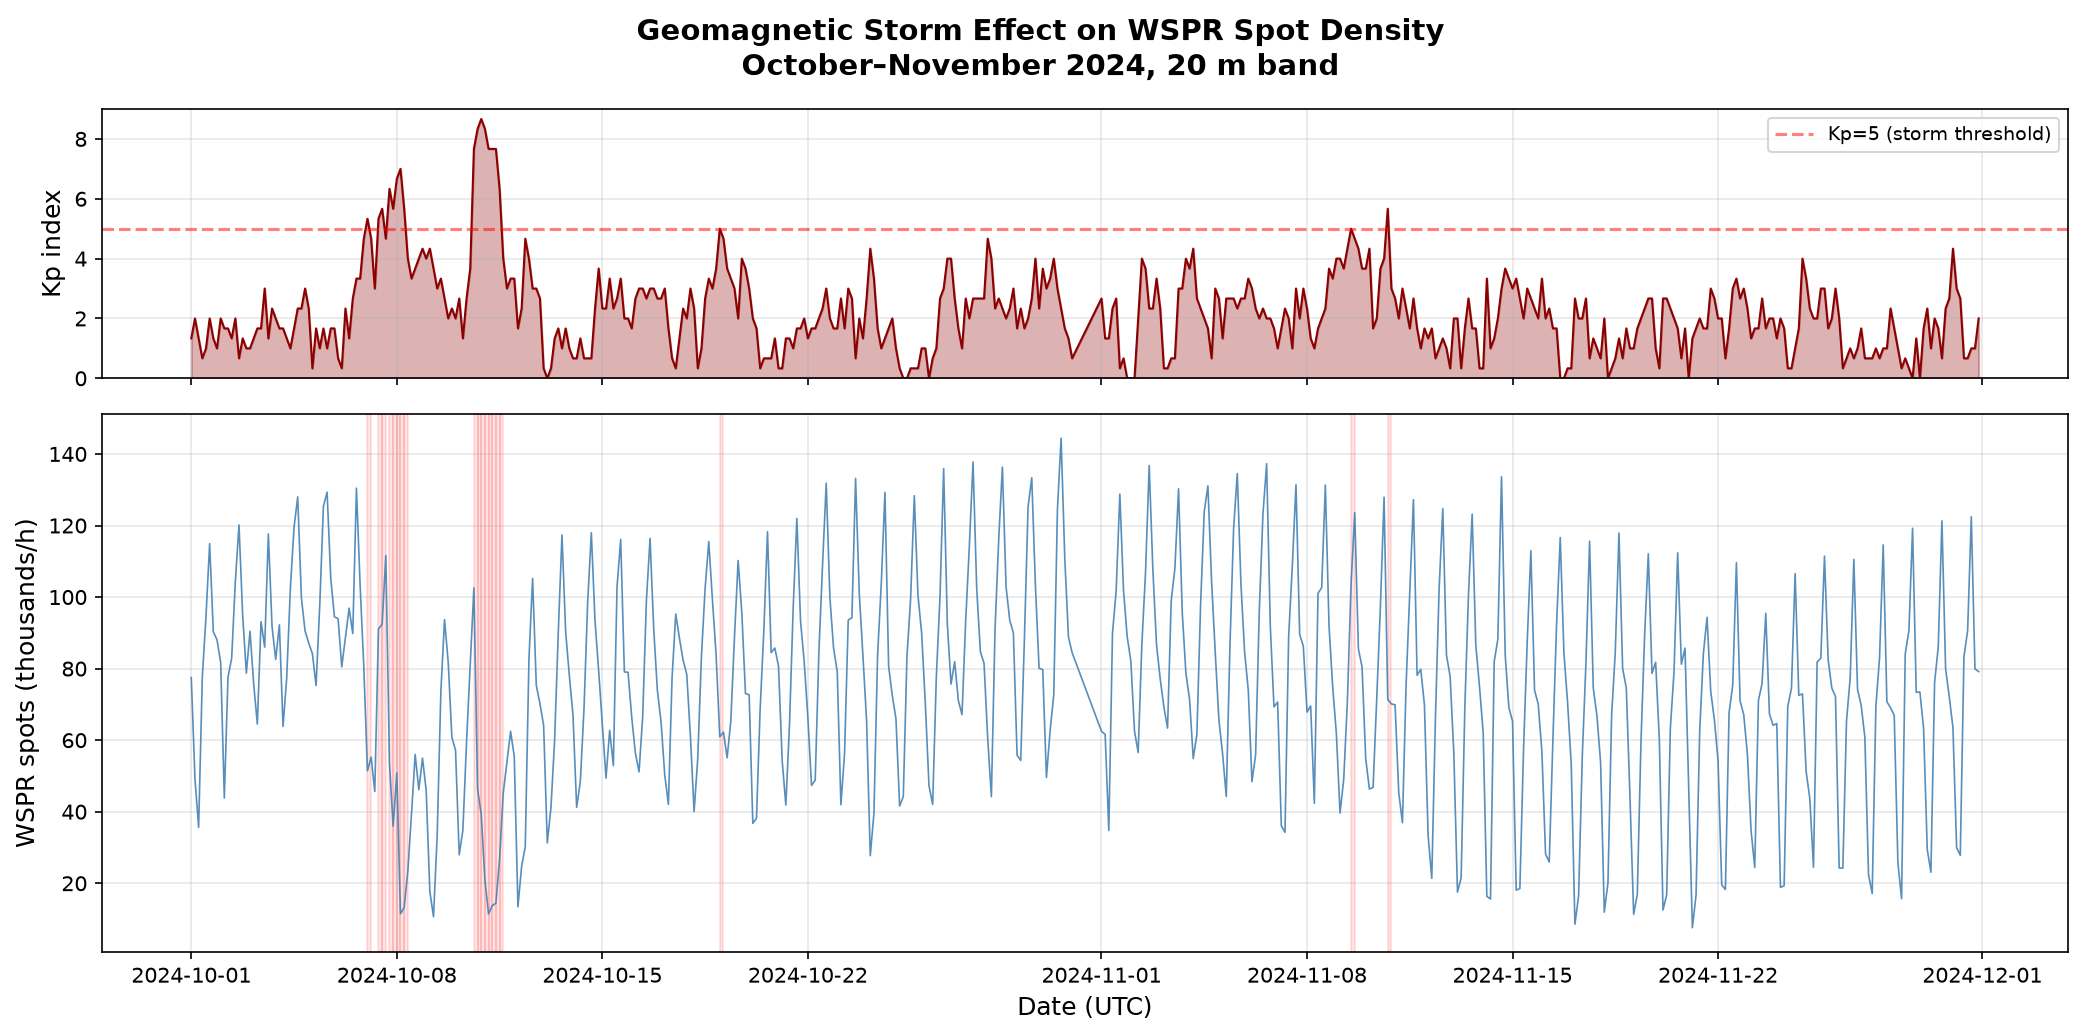
\includegraphics[width=\textwidth]{figures/fig1_kp_timeseries.png}
	\caption{Пример за два месяца: временной ряд индекса $Kp$ с наложением
		плотности WSPR-спотов (диапазон 20\,m, октябрь--ноябрь 2024 г.).
		Интервалы бурь ($Kp \ge 5$) выделены; подавление WSPR-спотов
		при повышенном $Kp$ визуально заметно.}
	\label{fig:timeseries}
\end{figure}

В Table~\ref{tab:main} представлен основной результат: вызванное бурями
снижение числа WSPR-спотов на всех трёх HF-диапазонах.

\begin{table}[h]
	\centering
	\footnotesize
	\setlength{\tabcolsep}{3pt}
	\caption{Основной результат: снижение числа WSPR-спотов во время бурь
		с $Kp \ge 5$ (18 месяцев, апрель 2024 -- сентябрь 2025).
		$N_{\text{storm}} = 198$ и $N_{\text{quiet}} = 3\,035$ для каждого
		диапазона в 3-часовых эпохах $Kp$. Исходное падение следует
		уравнению~\eqref{eq:drop} (исходные значения спотов) с 95\%
		доверительным интервалом (CI) блочного бутстрэпа (блоки по
		24 эпохи, 1\,000 перевыборок, seed 42). Скорректированное падение
		равно $100(e^{\beta}-1)$ из модели с отрицательным биномиальным
		распределением (уравнение~\eqref{eq:glm}) с 95\% CI,
		кластеризованным по эпизодам. $\Delta$ — исходная разность
		«буря минус спокойствие» (отрицательная для потери); её величина —
		абсолютное снижение, приведённое в Table~\ref{tab:baseline}.
		$p$-значения получены из блочного перестановочного теста остатков
		из раздела~3.3 (минимальное разрешимое $p$; нулевое число
		превышений).}
	\label{tab:main}
	\begin{tabular}{lcccr}
		\toprule
		Band & Raw drop (\%) [95\% CI] & Adj.\ drop (\%) [95\% CI]
		& $\Delta$ ($10^3$ spots/h) [95\% CI] & $p$ \\
		\midrule
		20\,m
		& $-27{,}7$ [$-36{,}6$, $-19{,}8$]
		& $-33{,}6$ [$-39{,}9$, $-26{,}7$]
		& $-20{,}4$ [$-26{,}8$, $-14{,}5$] & $\le 2\times10^{-5}$ \\
		40\,m
		& $-27{,}2$ [$-35{,}5$, $-19{,}3$]
		& $-27{,}1$ [$-33{,}2$, $-20{,}5$]
		& $-18{,}3$ [$-23{,}8$, $-12{,}9$] & $\le 2\times10^{-5}$ \\
		15\,m
		& $-38{,}7$ [$-48{,}9$, $-28{,}0$]
		& $-39{,}8$ [$-46{,}8$, $-31{,}8$]
		& $-5{,}2$ [$-6{,}7$, $-3{,}7$] & $\le 2\times10^{-5}$ \\
		\bottomrule
	\end{tabular}
\end{table}

Все три диапазона демонстрируют высокозначимое снижение плотности спотов
при $Kp \ge 5$ (блочная перестановка, \SI{50000}{iterations},
блок = 24 эпохи = 72\,h). Исходный эффект наиболее силён на 15\,m
(\SI{-38.7}{\percent}) и почти одинаков на 20\,m и 40\,m
(\SI{-27.7}{\percent} и \SI{-27.2}{\percent}). После поправки на
ковариаты падение на 20\,m возрастает по величине до \SI{-33.6}{\percent}
(95\% CI [\SI{-39.9}{\percent}, \SI{-26.7}{\percent}]): штормовые эпохи
перепредставлены в 00 UTC и в июне 2025 г., когда спокойный базовый
уровень 20\,m выше среднего (Table~\ref{tab:balance}). Оценка для 40\,m
практически не меняется (\SI{-27.1}{\percent}
[\SI{-33.2}{\percent}, \SI{-20.5}{\percent}]), а для 15\,m становится
\SI{-39.8}{\percent} ([\SI{-46.8}{\percent}, \SI{-31.8}{\percent}]).
Скорректированный порядок монотонен по частоте (15 $>$ 20 $>$ 40\,m),
в отличие от почти равных падений на 20 и 40\,m, рассчитанных по исходным
значениям. Все результаты
остаются значимыми после поправки на ложную частоту открытий (FDR)
Бенджамини--Хохберга для 6 тестов
($p_{\text{FDR}} \le 2 \times 10^{-5}$ для всех).

Анализ на основе $Dst$ даёт независимую проверку
(Table~\ref{tab:dst}); однако, поскольку в Table~\ref{tab:dst} приводятся
остаточные разности без члена дня недели, его значения $\Delta$ напрямую
не сравнимы с исходными дельтами $Kp$ в Table~\ref{tab:main}. Проверка
опирается на знак и значимость эффекта.

\begin{table}[h]
	\centering
	\caption{Проверка на основе $Dst$: $Dst < \SI{-50}{nT}$ против
		$Dst > \SI{-20}{nT}$. $N_{\text{Dst}}$ — общее число согласованных
		часов на диапазон ($N_{\text{storm}} = 471$ при
		$Dst < \SI{-50}{nT}$, $N_{\text{quiet}} = 8\,811$ при
		$Dst > \SI{-20}{nT}$). Остальные 3\,226 согласованных часов с
		$-50 \le Dst \le -20$\,nT исключены из этого сравнения.
		$\Delta$ — разность средних остатков (модель базового уровня
		месяц $\times$ час, без члена дня недели); $p$ — минимальное
		разрешимое значение (нулевое число превышений).}
	\label{tab:dst}
	\begin{tabular}{lrrl}
		\toprule
		Band  & $N_{\text{Dst}}$  & $\Delta_{\text{observed}}$ (spots/h)
		      & $p$-value (block)                                                    \\
		\midrule
		20\,m & 12\,508           & $-22\,081$                           & $\le 2 \times 10^{-5}$ \\
		40\,m & 12\,508           & $-15\,038$                           & $\le 2 \times 10^{-5}$ \\
		15\,m & 12\,508           & $-5\,143$                            & $\le 2 \times 10^{-5}$ \\
		\bottomrule
	\end{tabular}
\end{table}

\subsection{Масштабно-зависимый эффект}

Мы находим, что отклик WSPR возрастает с интенсивностью бури.
Figure~\ref{fig:scale} и Table~\ref{tab:scale} представляют анализ по
бинам $Kp$ за тренировочный период с использованием определения по исходным
значениям из уравнения~\eqref{eq:drop}.

\begin{figure}[t]
	\centering
	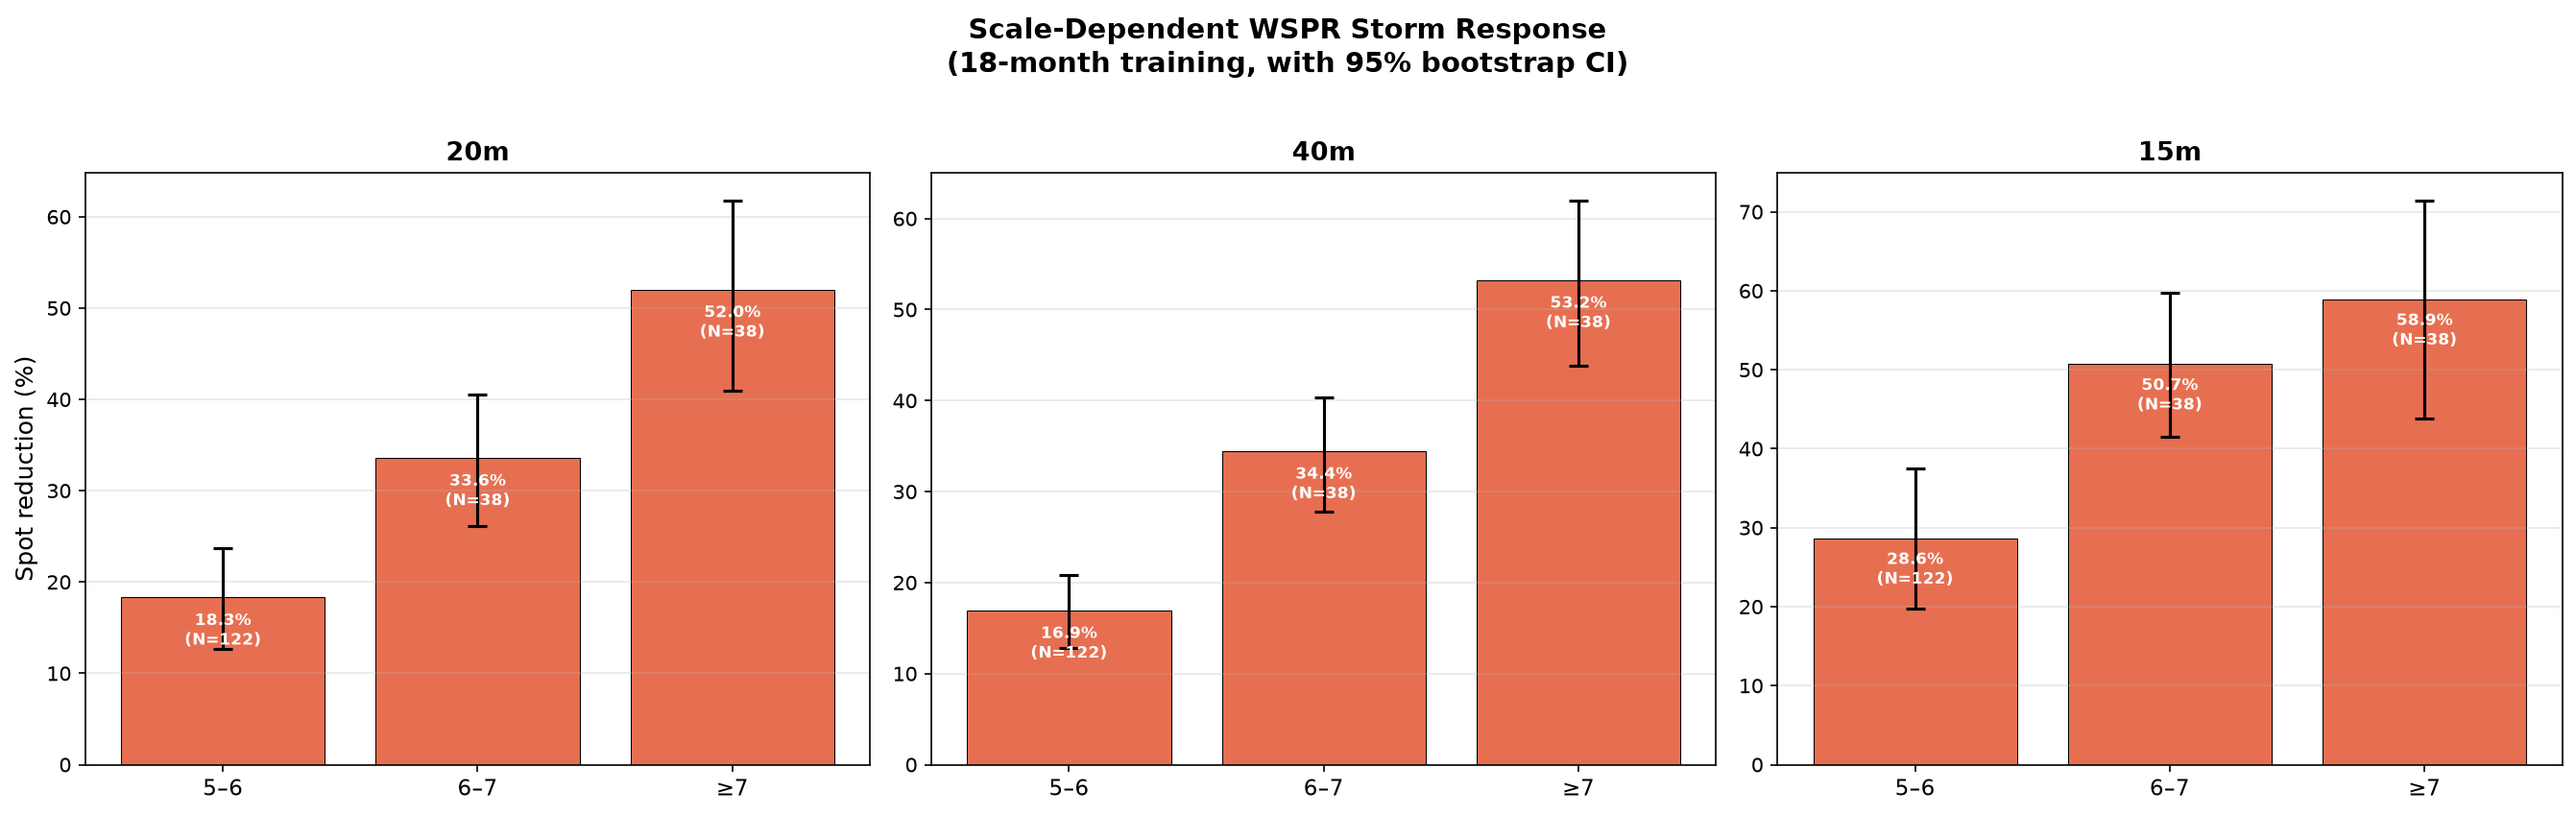
\includegraphics[width=\textwidth]{figures/fig2_scale_dependence.png}
	\caption{Масштабно-зависимое снижение числа WSPR-спотов: анализ по
		бинам для трёх HF-диапазонов (20\,m, 40\,m, 15\,m; 18-месячный
		тренировочный период). Снижение числа спотов (исходные значения,
		уравнение~\eqref{eq:drop}) показано для трёх штормовых бинов
		($Kp$ 5--6, 6--7, $\ge$7); спокойный референс ($Kp<3$) — нулевой
		уровень столбцов, а не отображаемый бин. Градиент по штормовым
		бинам согласуется с масштабно-зависимым откликом; бин с наибольшим
		$Kp$ разрежен (12 независимых эпизодов). Усы ошибок — 95\%
		iid-бутстрэп-интервалы; интервалы, кластеризованные по эпизодам,
		шире и приведены в Table~\ref{tab:episode} приложения.}
	\label{fig:scale}
\end{figure}

\begin{table}[h]
	\centering
	\footnotesize
	\setlength{\tabcolsep}{3pt}
	\caption{Масштабная зависимость: падение числа спотов (\%) по бинам
		$Kp$ для всех трёх диапазонов (тренировочный период, исходные значения
		спотов, уравнение~\eqref{eq:drop}); $N$ — число штормовых эпох
		в бине (общее для диапазонов), а число в скобках — число независимых
		штормовых эпизодов, дающих вклад. CI — 95\% iid-бутстрэп-интервалы
		(\SI{1000}{resamples}, seed 42), согласующиеся с усами ошибок на
		Figure~\ref{fig:scale}; кластерный бутстрэп по эпизодам даёт более
		широкие интервалы (Table~\ref{tab:episode} приложения).}
	\label{tab:scale}
	\begin{tabular}{lrrrr}
		\toprule
		$Kp$ bin & $N$ (episodes) & 20\,m drop (\%) [95\% CI]
		& 40\,m drop (\%) [95\% CI] & 15\,m drop (\%) [95\% CI] \\
		\midrule
		5--6     & 122 (54)
		& $-18{,}3$ [$-23{,}7$, $-12{,}7$]
		& $-16{,}9$ [$-21{,}1$, $-12{,}9$]
		& $-28{,}6$ [$-37{,}3$, $-20{,}0$] \\
		6--7     & 38 (22)
		& $-33{,}6$ [$-40{,}7$, $-26{,}6$]
		& $-34{,}4$ [$-40{,}5$, $-27{,}5$]
		& $-50{,}7$ [$-60{,}6$, $-40{,}9$] \\
		$\ge 6$  & 76 (23)
		& $-42{,}8$ [$-49{,}3$, $-35{,}9$]
		& $-43{,}8$ [$-49{,}3$, $-37{,}7$]
		& $-54{,}8$ [$-62{,}6$, $-46{,}3$] \\
		$\ge 7$  & 38 (12)
		& $-52{,}0$ [$-61{,}5$, $-41{,}0$]
		& $-53{,}2$ [$-62{,}1$, $-43{,}9$]
		& $-58{,}9$ [$-71{,}1$, $-44{,}5$] \\
		\bottomrule
	\end{tabular}
\end{table}

Падение приблизительно удваивается от $Kp = 5\text{--}6$
($\sim\SI{-18}{\percent}$) к $Kp = 6\text{--}7$ ($\sim\SI{-34}{\percent}$)
для 20\,m и 40\,m. При $Kp \ge 7$ снижение достигает
\SIrange{52}{59}{\percent} по всем диапазонам — сильное, но не на уровне
полного радиозатемнения (потеря $\SI{100}{\percent}$). Блочно-перестановочный
тест тренда по трём штормовым бинам значим для 20\,m ($p = 8\times10^{-4}$),
40\,m ($p \le 2\times10^{-4}$) и 15\,m ($p = 0.020$).

Масштабная зависимость подтверждается попарными блочно-перестановочными
тестами между бинами $Kp$ (все 9 комбинаций; Table~\ref{tab:pairwise}).
Пять из девяти сравнений выдерживают поправку Бенджамини--Хохберга;
четыре исключения — сравнения 15\,m $5\text{--}6$ против $\ge 7$ и
40\,m $5\text{--}6$ против $6\text{--}7$ (оба номинальных $p < 0.05$,
FDR $0{,}058$), а также два сравнения с наибольшим бином (20\,m и 15\,m
$6\text{--}7$ против $\ge 7$), где наибольший бин разрежен. Таким образом,
градиент статистически поддержан как тренд, но отдельные контрасты при
высоком $Kp$ разрешены не все. Наибольший бин содержит только 12
независимых эпизодов, а тест тренда на уровне эпизодов даёт Spearman
$\rho = -0.28$ ($p = 0.036$), $-0{,}24$ ($p = 0.064$) и $-0{,}27$
($p = 0.042$) для 20, 40 и 15\,m соответственно; поэтому тренд на уровне
эпизодов для 40\,m маргинален. Jackknife с исключением одного эпизода
сохраняет порядок трёх биновых падений во всех 58 повторностях для каждого
диапазона (Table~\ref{tab:episode} приложения), но это отражает
устойчивость порядка точек, а не значимость отдельных контрастов.

\begin{table}[h]
	\centering
	\caption{Попарный перестановочный тест между бинами $Kp$
		(тренировочный период). $\Delta$ в спотах/ч — разность средних
		остатков между двумя бинами (отдельная величина от исходной $\Delta$
		в Table~\ref{tab:main}). Столбец значимости номинальный; после
		поправки Бенджамини--Хохберга для девяти тестов 5 значимы при
		$\alpha = 0.05$ ($p_{\text{FDR}}$ четырёх исключений: 0,058,
		0,058, 0,097, 0,855).}
	\label{tab:pairwise}
	\begin{tabular}{llrrl}
		\toprule
		Band  & Comparison        & $\Delta$   & $p$-value & Significant?      \\
		\midrule
		20\,m & $Kp$ 5--6 vs 6--7 & $-7\,656$  & $0{,}0042$  & Yes ($p < 0.01$)  \\
		20\,m & $Kp$ 6--7 vs $7+$ & $-7\,315$  & $0{,}0860$  & No (trend)        \\
		20\,m & $Kp$ 5--6 vs $7+$ & $-14\,971$ & $0{,}0013$  & Yes ($p < 0.01$)  \\
		40\,m & $Kp$ 5--6 vs 6--7 & $-3\,664$  & $0{,}0450$  & Yes ($p < 0.05$)  \\
		40\,m & $Kp$ 6--7 vs $7+$ & $-9\,507$  & $0{,}0025$  & Yes ($p < 0.01$)  \\
		40\,m & $Kp$ 5--6 vs $7+$ & $-13\,171$ & $0{,}0001$  & Yes ($p < 0.001$) \\
		15\,m & $Kp$ 5--6 vs 6--7 & $-2\,228$  & $0{,}0032$  & Yes ($p < 0.01$)  \\
		15\,m & $Kp$ 6--7 vs $7+$ & $-195$     & $0{,}8547$  & No (saturation)   \\
		15\,m & $Kp$ 5--6 vs $7+$ & $-2\,423$  & $0{,}0422$  & Yes ($p < 0.05$)  \\
		\bottomrule
	\end{tabular}
\end{table}

\subsection{Частотная зависимость}

Частотная зависимость согласуется с двухмеханизменной структурой
(Figure~\ref{fig:freq}): 15\,m (\SI{-38.7}{\percent}) подвержен существенно
сильнее, чем 20\,m (\SI{-27.7}{\percent}) и 40\,m
(\SI{-27.2}{\percent}). После поправки на ковариаты порядок становится
монотонным (15\,m \SI{-39.8}{\percent}, 20\,m \SI{-33.6}{\percent},
40\,m \SI{-27.1}{\percent}), тогда как исходные падения на 20\,m и 40\,m
почти равны; это ожидаемо, если 20\,m получает дополнительный штраф по
MUF в дневном UT-окне, который при усреднении исходных значений частично
компенсируется более сильным ночным поглощением на 40\,m.

\begin{figure}[t]
	\centering
	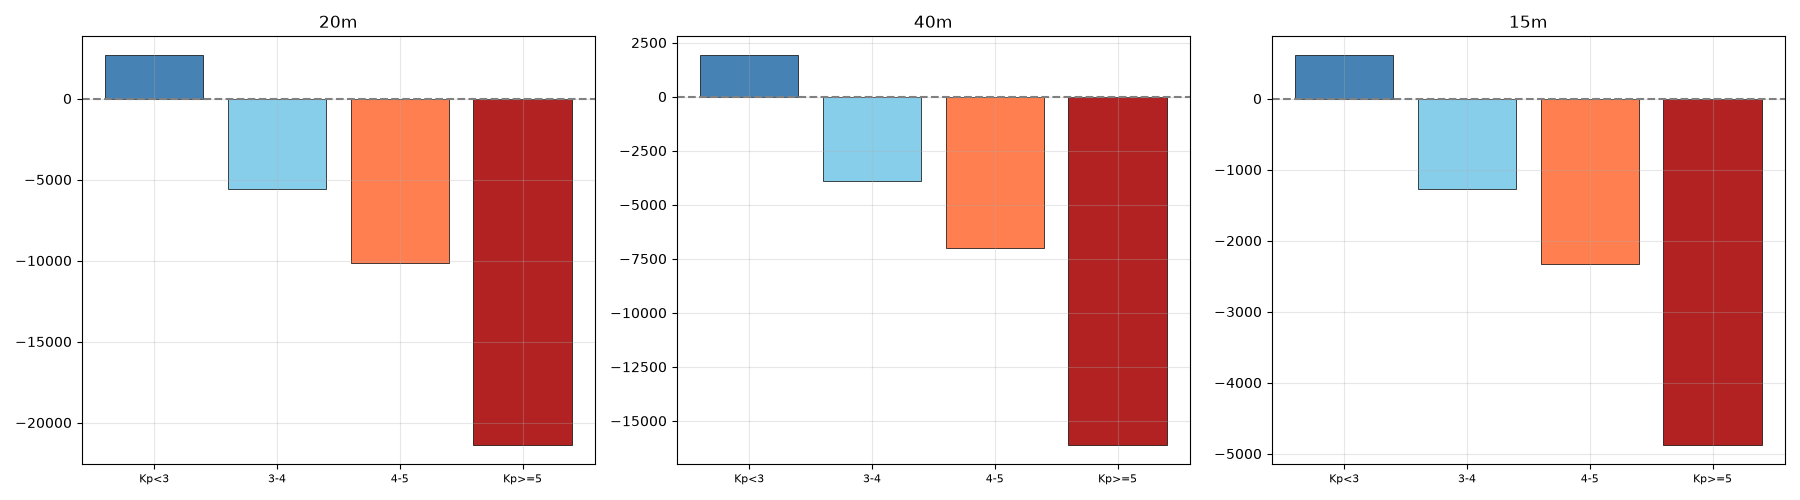
\includegraphics[width=0.85\textwidth]{figures/fig3_frequency_dependence.png}
	\caption{Частотная зависимость штормового отклика WSPR. Снижение числа
		спотов для трёх HF-диапазонов во время бурь с $Kp \ge 5$.
		Диапазон 15\,m показывает существенно более сильное подавление
		($\SI{-38.7}{\percent}$), чем 20\,m ($\SI{-27.7}{\percent}$)
		и 40\,m ($\SI{-27.2}{\percent}$), что согласуется
		с двухмеханизменной интерпретацией (снижение MUF на 15\,m,
		поглощение в слое D на 20\,m/40\,m).}
	\label{fig:freq}
\end{figure}

Эта картина согласуется с двумя различными физическими механизмами,
действующими одновременно:

\begin{enumerate}
	\item \textbf{Снижение MUF (диапазон 15\,m):} На 21\,MHz WSPR работает
	      вблизи типичной MUF для дневного UT-окна (\SIrange{14}{28}{MHz} в зависимости
	      от географической трассы и солнечных условий). Геомагнитная буря
	      снижает $f_oF_2$, опуская MUF ниже \SI{21}{MHz} на затронутых
	      трассах. В окне 12--18 UTC падение на 15\,m достигает
	      \SI{-48.9}{\percent}, что согласуется с MUF как основным
	      ограничением в дневном UT-окне.
	\item \textbf{Поглощение в слое D (диапазоны 20\,m / 40\,m):} Оба
	      диапазона работают существенно ниже типичной MUF, поэтому их
	      основная чувствительность связана с недевиационным поглощением
	      в слое D, которое масштабируется как $\propto 1/f^2$. Однако
	      суммарные падения почти равны ($\SI{-27.7}{\percent}$ против
	      $\SI{-27.2}{\percent}$), что, по-видимому, противоречит
	      масштабированию $1/f^2$ (40\,m на \SI{7}{MHz} должен быть
	      затронут примерно в 4 раза сильнее, чем 20\,m на \SI{14}{MHz}).
\end{enumerate}

Этот кажущийся парадокс разрешается при учёте зависимости двух механизмов
от времени суток (см. раздел~\ref{sec:daynight}).

Эти атрибуции согласуются с указанными механизмами, но не устанавливают
их однозначно; прямое разделение эффектов MUF и поглощения требует анализа
SNR или фазы, выходящего за рамки этого исследования.

\subsection{Асимметрия UT-окон}
\label{sec:daynight}

Разложение по UT-окнам (Figure~\ref{fig:daynight}) показывает, что почти
равенство суммарных падений на 20\,m и 40\,m возникает из-за двух
механизмов, действующих противоположно в течение суточного цикла
(Table~\ref{tab:daynight}).

\begin{table}[h]
	\centering
	\caption{Разложение падения числа спотов по UT-окнам
		(тренировочный период). Точечные оценки и 95\% CI из
		бутстрэп-перевыборки (\SI{1000}{resamples});
		$N_{\text{storm}} / N_{\text{quiet}}$ указаны. Строки «все часы» —
		результат блочной перестановки (наблюдаемое, без CI). Строки для дневного и ночного UT-окон охватывают 111 из 198 штормовых эпох и 1\,466
		из 3\,035 спокойных эпох; остальные выходят за пределы окон
		12--18 и 0--6 UTC.}
	\label{tab:daynight}
	\begin{tabular}{llrrl}
		\toprule
		Band & Period & Drop (\%) & 95\% CI & $N_{\text{storm}}/N_{\text{quiet}}$ \\
		\midrule
		20\,m & UT-day    & $\SI{-28.7}{\percent}$ & [$\SI{-36.4}{\percent}$, $\SI{-21.7}{\percent}$] & 53/732  \\
		20\,m & UT-night  & $\SI{-24.8}{\percent}$ & [$\SI{-33.9}{\percent}$, $\SI{-16.8}{\percent}$] & 58/734  \\
		20\,m & All    & $\SI{-27.7}{\percent}$ & --- & 198/3035 \\
		\midrule
		40\,m & UT-day    & $\SI{-20.7}{\percent}$ & [$\SI{-28.2}{\percent}$, $\SI{-13.7}{\percent}$] & 53/732  \\
		40\,m & UT-night  & $\SI{-30.2}{\percent}$ & [$\SI{-36.4}{\percent}$, $\SI{-24.6}{\percent}$] & 58/734  \\
		40\,m & All    & $\SI{-27.2}{\percent}$ & --- & 198/3035 \\
		\midrule
		15\,m & UT-day    & $\SI{-48.9}{\percent}$ & [$\SI{-58.1}{\percent}$, $\SI{-39.6}{\percent}$] & 53/732  \\
		15\,m & UT-night  & $\SI{-18.7}{\percent}$ & [$\SI{-34.4}{\percent}$, $\SI{-4.4}{\percent}$]  & 58/734  \\
		15\,m & All    & $\SI{-38.7}{\percent}$ & --- & 198/3035 \\
		\bottomrule
	\end{tabular}
\end{table}

\textbf{Дневное UT-окно} (12--18 UTC): MUF высока, а 40\,m работает намного ниже
неё. Слой D, поддерживаемый солнечным UV/EUV, вызывает поглощение на обоих
диапазонах, но подавление MUF во время бурь дополнительно влияет на 20\,m,
который работает ближе к потолку MUF. Результат: 20\,m падает сильнее
($\SI{-28.7}{\percent}$), чем 40\,m ($\SI{-20.7}{\percent}$).

\textbf{Ночное UT-окно} (0--6 UTC): Слой D, поддерживаемый Солнцем, исчезает
в течение минут после заката (электронная плотность падает до
$\sim 10^3$\,cm$^{-3}$). Однако во время геомагнитных бурь высыпание
энергичных частиц повторно ионизирует область D независимо от солнечного
излучения: авроральное поглощение от электронов \SIrange{30}{300}{keV}
\citep{hargreaves1969,royrvik1977} и поглощение в полярной шапке (PCA)
от солнечных протонов \SIrange{1}{30}{MeV} \citep{reid1974}. Возникающее
поглощение в слое D сохраняет масштабирование $1/f^2$: 40\,m испытывает
примерно в 4 раза большее поглощение на единицу электронной плотности,
чем 20\,m. Результат: 40\,m падает сильнее ($\SI{-30.2}{\percent}$),
чем 20\,m ($\SI{-24.8}{\percent}$).

Эффект ночного UT-окна на 15\,m меньше и менее определён, чем эффект дневного UT-окна
($\SI{-18.7}{\percent}$, 95\% CI
[$\SI{-34.4}{\percent}$, $\SI{-4.4}{\percent}$]), что согласуется
с преимущественным отсутствием солнечного слоя D в окне 0--6 UTC.

При интегрировании за 24 часа штраф MUF в дневном UT-окне для 20\,m и более
сильное авроральное/PCA-поглощение в ночном UT-окне для 40\,m могут компенсировать
друг друга, создавая наблюдаемое почти равенство суммарных падений,
рассчитанных по исходным значениям.
Эта картина согласуется с гипотезой двух механизмов, но не является
единственным предсказанием: другие комбинации суточного покрытия сети
и штормового поглощения могли бы дать аналогичный кроссовер.

Поскольку WSPR — глобальная сеть, окна 12--18 UTC и 0--6 UTC не
соответствуют одновременным местным дню и ночи. Поэтому их следует
интерпретировать как композиты UT-секторов. Для окончательной атрибуции
день/ночь требуется местное солнечное время или интегральная по трассе
солнечная освещённость.

Окна 12--18 и 0--6 UTC были зафиксированы до помесячного анализа как два
6-часовых сектора с наибольшим числом штормовых эпох; они являются
поисковыми композитами UT-секторов и не входили в подтверждающее
семейство множественных сравнений. Помесячное сравнение носит описательный
характер и не скорректировано на множественность.


\begin{figure}[t]
	\centering
	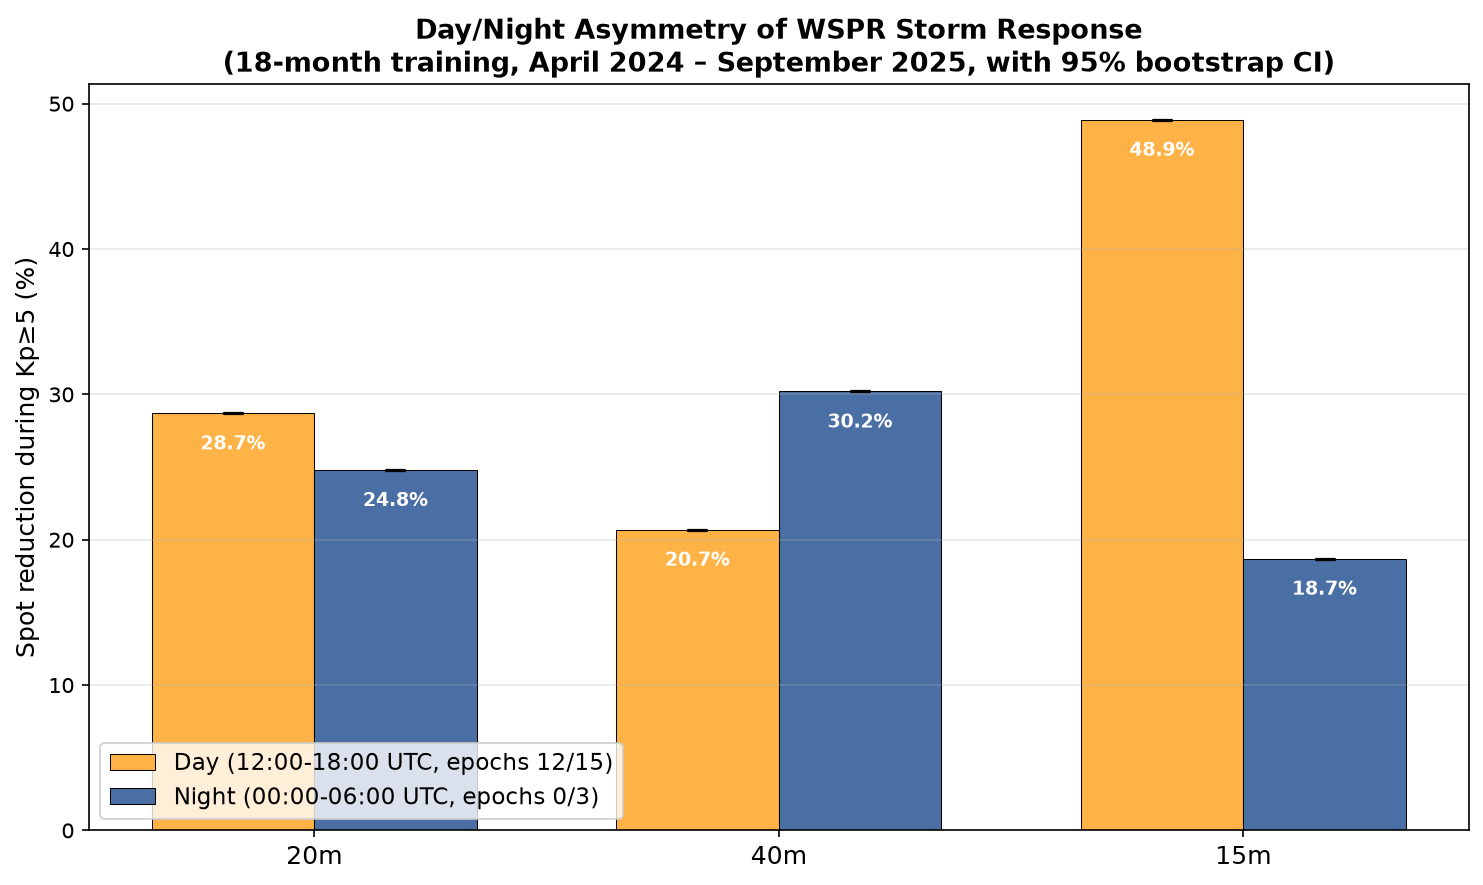
\includegraphics[width=\textwidth]{figures/fig4_day_night_asymmetry.png}
	\caption{Асимметрия UT-окон штормового отклика WSPR. Помесячное падение
		числа спотов на 40\,m, разложенное по дневному UT-окну (12--18 UTC, эпохи
		12/15) и ночному UT-окну (0--6 UTC, эпохи 0/3). Падения в ночном UT-окне
		превышают падения в дневном UT-окне во всех 8 тренировочных месяцах
		с достаточными штормовыми данными ($\ge$3 штормовых эпохи на окно),
		что согласуется с перемежающимся авроральным поглощением
		и поглощением в полярной шапке. Два окна были зафиксированы до
		помесячного анализа как 6-часовые секторы с наибольшим числом
		штормовых эпох; это композиты UT-секторов, а не местный день/ночь.}
	\label{fig:daynight}
\end{figure}

Помесячный анализ тренировочного периода показывает, что для 40\,m
ночное UT-окно $>$ дневное UT-окно во всех 8 месяцах с достаточными данными,
удовлетворяющими критерию $\ge$3 эпох ($\ge$3 штормовых эпохи в каждом
UT-окне), что согласуется с перемежающимся характером высыпания частиц:
механизм требует специфических морфологий бурь, которые присутствуют
не в каждом событии.

\subsection{Независимое воспроизведение}

Трёхмесячный отложенный период (январь--март 2026) обеспечивает независимую
проверку как основного эффекта, так и его масштабной зависимости
(Table~\ref{tab:heldout}).

\begin{table}[h]
	\centering
	\caption{Независимое воспроизведение: отложенный период
		(январь--март 2026). Числа из живой выгрузки \texttt{wspr.live}
		от 2026-10-15; более ранний архивный снимок давал меньшие $N$
		и падения. Исходное падение следует уравнению~\eqref{eq:drop}
		по исходным числам спотов с 95\% CI блочного бутстрэпа;
		скорректированное падение — из модели с отрицательным
		биномиальным распределением (уравнение~\eqref{eq:glm}) с 95\% CI,
		кластеризованным по эпизодам. $p$-значения получены из блочного
		перестановочного теста остатков из раздела~3.3. См. ограничение
		«архив против живой базы» в разделе~5.5.
		$N_{\text{total}} = 720$, $N_{\text{storm}} = 47$ и
		$N_{\text{quiet}} = 439$ одинаковы для всех диапазонов, поскольку
		классификация $Kp$ общая.}
	\label{tab:heldout}
	\begin{tabular}{lccr}
		\toprule
		Band & Raw drop (\%) [95\% CI] & Adj.\ drop (\%) [95\% CI] & $p$ \\
		\midrule
		20\,m
		& $-26{,}7$ [$-41{,}5$, $-3{,}4$]
		& $-19{,}1$ [$-32{,}2$, $-3{,}6$] & $\le 2 \times 10^{-5}$ \\
		40\,m
		& $-29{,}0$ [$-40{,}8$, $-14{,}0$]
		& $-21{,}2$ [$-32{,}6$, $-7{,}7$] & $2 \times 10^{-4}$ \\
		15\,m
		& $-22{,}1$ [$-42{,}5$, $22{,}8$]
		& $-23{,}4$ [$-40{,}4$, $-1{,}7$] & $8 \times 10^{-5}$ \\
		\bottomrule
	\end{tabular}
\end{table}

Все три диапазона показывают отрицательные падения, значимые по блочному
перестановочному тесту остатков из раздела~3.3: $\SI{-26.7}{\percent}$
(20\,m, $p \le 2 \times 10^{-5}$), $\SI{-29.0}{\percent}$ (40\,m,
$p = 2 \times 10^{-4}$) и $\SI{-22.1}{\percent}$ (15\,m,
$p = 8 \times 10^{-5}$). $p$-значения проверяют ряд остатков, тогда как
доверительный интервал абсолютного снижения в Table~\ref{tab:baseline}
вычислен по исходным числам спотов; для 15\,m этот интервал всё ещё включает
ноль, что отражает меньший размер эффекта, а не недостаток объёма выборки
($N_{\text{storm}} = 47$ общее для диапазонов).

После поправки на ковариаты падения на отложенном периоде составляют
\SI{-19.1}{\percent} (20\,m), \SI{-21.2}{\percent} (40\,m) и
\SI{-23.4}{\percent} (15\,m), все с CI, исключающими ноль
(Table~\ref{tab:heldout}). Они меньше оценок тренировочного периода
(исходные \SI{-27.7}{\percent}, \SI{-27.2}{\percent}, \SI{-38.7}{\percent};
скорректированные \SI{-33.6}{\percent}, \SI{-27.1}{\percent},
\SI{-39.8}{\percent}), поэтому воспроизведение является направленным
и значимым, но не количественно точным. Тем не менее исходные процентные
падения на 20\,m и 40\,m сопоставимы с тренировочными; падение на 15\,m
на отложенном периоде меньше тренировочного значения при широком
доверительном интервале. Абсолютные снижения составляют
$\SI{-22482}{spots/h}$ (20\,m), $\SI{-26287}{spots/h}$ (40\,m) и
$\SI{-3627}{spots/h}$ (15\,m); см. раздел~\ref{sec:invariant}.

При сопоставлении по силе бури масштабная зависимость направленно
согласуется: при $Kp = 6\text{--}7$ тренировочные и отложенные падения
совпадают в пределах коэффициентов 1,01--1,12 (Table~\ref{tab:scale_rep}),
исходя из $N_{\text{storm}} = 10$ на диапазон в отложенном периоде.

\begin{table}[h]
	\centering
	\caption{Воспроизведение масштабной зависимости: тренировочный период
		против отложенного при $Kp = 6\text{--}7$. Числа отложенного периода
		из живой выгрузки \texttt{wspr.live} от 2026-10-15
		($N_{\text{storm}} = 10$ на диапазон). Это направленная проверка,
		а не достаточно мощное подтверждение.}
	\label{tab:scale_rep}
	\begin{tabular}{llll}
		\toprule
		Band  & Training drop (\%)     & Held-out drop (\%)     & Ratio (H/T) \\
		\midrule
		20\,m & $\SI{-33.6}{\percent}$ & $\SI{-37.4}{\percent}$ & 1,11        \\
		40\,m & $\SI{-34.4}{\percent}$ & $\SI{-34.6}{\percent}$ & 1,01        \\
		15\,m & $\SI{-50.7}{\percent}$ & $\SI{-57.0}{\percent}$ & 1,12        \\
		\bottomrule
	\end{tabular}
\end{table}

Частотная зависимость и асимметрия UT-окон независимо не воспроизводятся
в трёхмесячном отложенном окне, что ожидаемо: частотная зависимость
требует больших штормовых выборок для разделения двух механизмов,
а асимметрия UT-окон — специфических морфологий бурь (высыпания энергичных
частиц), которые не преобладали в этом конкретном трёхмесячном интервале.

В частности, исходный частотный порядок инвертируется между двумя периодами:
в тренировочном падения равны \SI{-38.7}{\percent} (15\,m),
\SI{-27.7}{\percent} (20\,m) и \SI{-27.2}{\percent} (40\,m), тогда как
в отложенном окне они равны \SI{-22.1}{\percent} (15\,m),
\SI{-26.7}{\percent} (20\,m) и \SI{-29.0}{\percent} (40\,m)
(Table~\ref{tab:heldout}). После поправки на ковариаты порядок на
отложенном периоде становится \SI{-23.4}{\percent} (15\,m),
\SI{-21.2}{\percent} (40\,m) и \SI{-19.1}{\percent} (20\,m). Это
возвращает 15\,m на позицию наиболее затронутого диапазона, в отличие
от исходного порядка отложенного периода, но порядок 20\,m/40\,m остаётся
обратным относительно скорректированного тренировочного порядка
(15 $>$ 20 $>$ 40\,m); доверительные интервалы широко перекрываются.
Три фактора могут объяснить исходную инверсию, не противореча
двухмеханизменной интерпретации. Во-первых, статистическая мощность:
доступно только 47 штормовых эпох, а падение на 15\,m на отложенном
периоде — самое слабое из трёх (его исходный 95\% CI в
Table~\ref{tab:baseline} включает ноль), поэтому порядок точечных оценок
плохо ограничен. Во-вторых, сезонный состав: тренировочный период
охватывает все четыре сезона, тогда как январь--март содержит только
позднезимние и ранневесенние бури с иной климатологией MUF в дневном UT-окне
и более короткими днями. В-третьих, Es-слой: часть летних
тренировочных спотов на 15\,m приходит через Es, а не через
распространение в слое F (раздел~5.5), поэтому тренировочная и отложенная
выборки на 15\,m не являются строго сопоставимыми, а направление этого
смещения нельзя определить только по числам спотов. Таким образом,
отложенное окно согласуется с частотным порядком, но не подтверждает его
независимо; для подтверждения требуется более длинное окно
воспроизведения, охватывающее несколько сезонов.

\subsection{Абсолютное снижение и зависимость от размера сети}
\label{sec:invariant}

\begin{figure}[t]
	\centering
	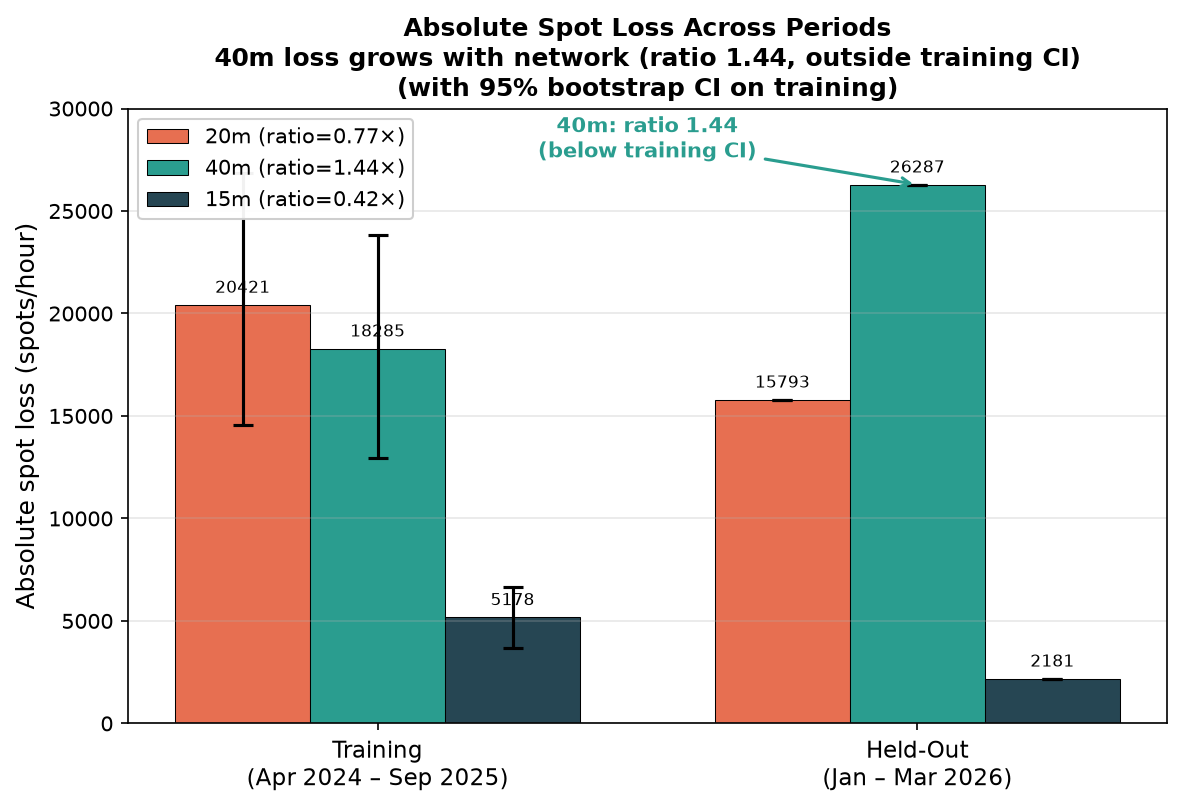
\includegraphics[width=0.85\textwidth]{figures/fig5_baseline_invariance.png}
	\caption{Абсолютное снижение числа спотов между периодами. Сравнение
		абсолютного снижения числа WSPR-спотов во время бурь между
		тренировочным (18 месяцев) и отложенным (3 месяца) периодами для всех
		трёх диапазонов. Тренировочная оценка для 40\,m
		($\SI{-18285}{spots/h}$) первоначально совпадала с отложенным снимком
		($\SI{-18304}{spots/h}$); обновлённая выгрузка (2026-10-15) даёт
		$\SI{-26287}{spots/h}$ (отношение 1,44, 95\% CI [0,65, 2,33]);
		точечная оценка 1,44 превышает ожидаемое масштабирование
		$\approx$1,35 при росте спокойного базового уровня на
		$\SI{+35}{\percent}$, но широкий CI совместим как с пропорциональным
		ростом, так и с инвариантностью; процентные падения остаются более
		устойчивой метрикой.}
	\label{fig:baseline}
\end{figure}

Центральный вопрос для оперативного мониторинга — устойчиво ли абсолютное
снижение спотов (спотов/ч) при росте сети WSPR.
Table~\ref{tab:baseline} сравнивает абсолютные и относительные падения
между тренировочным и отложенным периодами.

\begin{table}[h]
	\centering
	\small
	\setlength{\tabcolsep}{5pt}
	\caption{Абсолютное снижение числа спотов между периодами (единицы: спотов/ч).
		Точечные оценки тренировочного и отложенного периодов с 95\%
		CI блочного бутстрэпа (блоки по 24 эпохи = 72\,h, 1000 перевыборок,
		seed 42): тренировочный CI из живого прогона 2026-10-13 (идентичен
		пересчёту по замороженному parquet), значения и CI отложенного
		периода — из живой выгрузки \texttt{wspr.live} от 2026-10-15.
		Обновлённое значение для 40\,m ($\SI{-26287}{spots/h}$, отношение
		1,44, 95\% CI [0,65, 2,33]) лежит вне тренировочного точечного CI,
		но его собственный CI перекрывается с ним. Точечная оценка 1,44
		превышает ожидаемое масштабирование $\approx$1,35 при росте спокойного
		базового уровня на $\SI{+35}{\percent}$, но широкий CI отношения
		совместим как с пропорциональным ростом, так и с инвариантностью.
		Процентные падения остаются более устойчивой метрикой.\protect\footnotemark{}}
	\label{tab:baseline}
	\begin{tabular}{lccc}
		\toprule
		Band  & Training abs.\ loss [95\% CI] & Held-out abs.\ loss [95\% CI]
		& Ratio (H/T) [95\% CI] \\
		\midrule
		20\,m & $\num{-20421}$ [$\num{-26834}$, $\num{-14544}$]
		& $\num{-22482}$ [$\num{-35044}$, $\num{-2938}$]
		& 1,10 [0,18, 1,94] \\
		40\,m & $\num{-18285}$ [$\num{-23807}$, $\num{-12930}$]
		& $\num{-26287}$ [$\num{-37144}$, $\num{-12472}$]
		& \textbf{1,44} [0,65, 2,33] \\
		15\,m & $\num{-5178}$ [$\num{-6671}$, $\num{-3684}$]
		& $\num{-3627}$ [$\num{-7172}$, $\num{3738}$]
		& 0,70 [0,05, 1,57] \\
		\bottomrule
	\end{tabular}
\end{table}
\footnotetext{Значения и CI отложенного периода из живой выгрузки \texttt{wspr.live} от 2026-10-15; CI отношения из \texttt{scripts/abs\_loss\_ratio\_ci.py} (блочный бутстрэп, блоки по 24 эпохи, 1000 перевыборок, seed 42); см. \texttt{audit/FINDING\_HELDOUT\_LIVE\_2026-10-13.md}.}

{\sloppy Начальная точечная оценка тренировочного периода для 40\,m
(Figure~\ref{fig:baseline}; $\SI{-18285}{spots/h}$; 95\% CI блочного
бутстрэпа $[\SI{-23807}{spots/h},\, \SI{-12930}{spots/h}]$) и первый
снимок отложенного периода ($\SI{-18304}{spots/h}$) согласовывались
с постоянным абсолютным снижением, несмотря на рост спокойного базового
уровня на $\SI{+35}{\percent}$ из-за роста сети. Сначала мы
интерпретировали это как свидетельство того, что уязвимые к бурям
трассы распространения образуют структурно ограниченную популяцию,
которая не увеличивается при добавлении станций в уже покрытые
регионы.\par}

Однако отложенный период обслуживается живой базой \texttt{wspr.live},
которая непрерывно обновляется по мере загрузки операторами отложенных
журналов. Повторная выгрузка 2026-10-15 даёт существенно большую
выборку отложенного периода для 40\,m ($N = 720$ эпох,
$N_{\text{storm}} = 47$, по сравнению с $N_{\text{total}} = 648$,
$N_{\text{storm}} = 38$ в архивном снимке) и абсолютное снижение
$\SI{-26287}{spots/h}$ (95\% CI блочного бутстрэпа
$[-\SI{37144}{spots/h},\, -\SI{12472}{spots/h}]$), которое лежит
\emph{ниже} нижней границы тренировочного CI. Это точечное сравнение:
тренировочный и отложенный CI перекрываются, поэтому это не формальный
тест на равенство. Отношение отложенный / тренировочный при расширенных
данных равно 1,44 (95\% бутстрэп-CI [0,65, 2,33]), а не 1,00.

Поэтому мы не утверждаем инвариантность базового уровня как установленный
результат. Остаются возможными два объяснения, которые нельзя полностью
разделить на имеющихся данных: (i) абсолютное снижение растёт с размером
сети и штормовым покрытием или (ii) архивный снимок отложенного периода
был смещён вниз из-за эффекта задержки загрузки в базе
\texttt{wspr.live}. Обновлённые данные совместимы с количественной формой
(i) — пропорциональным масштабированием: наблюдаемое отношение равно
1,44; это точечная оценка, превышающая ожидаемое масштабирование
($\approx$1,35), если процентное падение постоянно, а спокойный
базовый уровень вырос на $\SI{+35}{\percent}$, но широкий
бутстрэп-CI отношения [0,65, 2,33] совместим как с пропорциональным
ростом, так и с инвариантностью (он также включает единицу, поэтому
строгую инвариантность тоже нельзя исключить). Поэтому мы рассматриваем
абсолютное снижение как совместимое с масштабированием, связанным с сетью,
но не установленное окончательно, и отмечаем, что процентные падения
остаются более устойчивой метрикой для межпериодных сравнений.
Различение (i) и (ii) потребовало бы замороженного снимка данных на момент
анализа, который не был сохранён для исходного отложенного периода.

Точечные оценки тренировочного периода различаются по диапазонам
(40\,m: $\SI{-18285}{spots/h}$; 20\,m: $\SI{-20421}{spots/h}$;
15\,m: $\SI{-5178}{spots/h}$); отношения отложенный / тренировочный
(0,70--1,44) неточны и охватывают как единицу, так и пропорциональное
масштабирование, поэтому мы приводим абсолютные значения как описательные
величины, а не как метрику, инвариантную к размеру сети.


%=============================================================
\section{Обсуждение}
%=============================================================

\subsection{Физические механизмы}

Наблюдаемый отклик WSPR согласуется со стандартной картиной ионосферных
штормовых эффектов, но многодиапазонное покрытие выявляет два отдельных
механизма, которые теперь можно различить:

\textbf{Цепочка подавления MUF:} рост $Kp$ $\rightarrow$ усиленная
магнитосферная конвекция $\rightarrow$ джоулев нагрев в авроральном овале
$\rightarrow$ повышение температуры нейтральной атмосферы $\rightarrow$
изменения состава (рост отношения N$_2$/O) $\rightarrow$ повышение скорости
рекомбинации $\rightarrow$ снижение $f_oF_2$ $\rightarrow$ падение MUF ниже
рабочей частоты на затронутых трассах $\rightarrow$ сигнал больше не
отражается $\rightarrow$ меньше WSPR-спотов. Этот механизм преимущественно
влияет на самый высокий диапазон 15\,m (\SI{-38.7}{\percent}).

\textbf{Цепочка поглощения в слое D:} рост $Kp$ $\rightarrow$ высыпание
частиц (электроны и протоны) $\rightarrow$ усиление ионизации области D
$\rightarrow$ недевиационное HF-поглощение $\propto 1/f^2$ $\rightarrow$
ослабление сигнала ниже порога декодирования WSPR $\rightarrow$ меньше
спотов. Этот механизм влияет на все диапазоны, но наиболее заметен на
20\,m и 40\,m, причём поглощение на 40\,m примерно в 4 раза сильнее на
единицу электронной плотности.

Почти равенство суммарных падений на 20\,m и 40\,m, рассчитанных по исходным
значениям, не противоречит
масштабированию поглощения $1/f^2$: подавление MUF дополнительно штрафует
20\,m в дневном UT-окне, а вызванное частицами поглощение в слое D дополнительно
штрафует 40\,m в ночном UT-окне. После поправки на ковариаты падение на 20\,m
фактически больше падения на 40\,m, что согласуется с этой компенсацией.
Разложение по UT-окнам (раздел~\ref{sec:daynight}) указывает, что оба
механизма могут действовать одновременно и проявляются при разделении
данных по времени суток.

Прямая проверка канала SNR информативна. Среди декодированных спотов
среднее SNR, взвешенное по спотам, во время бурь отличается от спокойного
периода всего на $+\SI{0.25}{dB}$ (15\,m, 95\% CI [0,11, 0,38]),
$-\SI{0.22}{dB}$ (20\,m, [-0,36, -0,07]) и $-\SI{0.41}{dB}$ (40\,m,
[-0,56, -0,26]) после поправки на месяц, UT-час и день недели (Таблица~A\ref{tab:snr}).
Поскольку недекодированные сигналы отсутствуют в этом
распределении, почти инвариантность означает, что большая часть снижения
счёта происходит из-за трасс, которые падают ниже порога декодирования или
исчезают, а не из-за равномерного снижения SNR выживших спотов. Это само
по себе не различает снижение MUF и поглощение; оба механизма удаляли бы
маргинальные трассы из декодированной выборки.

Грубое разложение по длине трассы (почасовые счётчики, разбитые по
расстоянию большого круга; Table~\ref{tab:distance} приложения) показывает,
что отклик неоднороден по длинам трасс. На 20\,m падение составляет
\SI{-23.4}{\percent} на трассах 0--2\,000\,km и \SI{-60.8}{\percent} на
трассах 5\,000--10\,000\,km; на 15\,m соответствующие значения
\SI{-35.7}{\percent} и \SI{-56.0}{\percent}, а на 40\,m
\SI{-23.8}{\percent} и \SI{-53.5}{\percent}. Бины длинных трасс содержат
только 3--13\% штормовых спотов, поэтому их CI широки, но направление
согласуется с ростом интегрального по трассе поглощения и деградации MUF
с длиной трассы. Это прокси расстояния, а не разложение по широте или
местному времени; координаты передатчика и приёмника и геометрия трасс
остаются для будущей работы.

\subsection{Масштабная зависимость и нелинейный отклик ионосферы}

Рост падения числа спотов с $Kp$ — центральный результат этого
исследования. Физическая основа этой нелинейности лежит в связанном отклике
системы ионосфера--термосфера:

\begin{itemize}
	\item Скорость джоулева нагрева пропорциональна $\Sigma_P \cdot E^2$,
	      где $\Sigma_P$ — педерсеновская проводимость, а $E$ — электрическое
	      поле конвекции. И $\Sigma_P$ (усиливается высыпанием частиц),
	      и $E$ (усиливается более сильной магнитосферной конвекцией) растут
	      с $Kp$, давая сверхлинейную скорость нагрева.
	\item Истощение $f_oF_2$ насыщается при сильных бурях ($Kp \ge 6$):
	      слой F2 приближается к химическому равновесию, где скорости
	      рождения и рекомбинации балансируются. Это может объяснять,
	      почему падения на 15\,m похожи при $Kp$ 6--7 (\SI{-51}{\percent})
	      и $Kp \ge 7$ (\SI{-59}{\percent}), и почему попарный тест между
	      этими бинами незначим ($p = 0.8547$ для 15\,m).
\end{itemize}

Практическое следствие: для существенного нарушения HF на средних
диапазонах (20\,m и 40\,m) требуется $Kp \ge 6$, тогда как более низкое
$Kp = 5\text{--}6$ даёт лишь умеренные снижения $\sim\SI{-18}{\percent}$.
Этот порог зависит от диапазона: на 15\,m $Kp = 5\text{--}6$ уже даёт
\SI{-28.6}{\percent}. Для сильного нарушения, превышающего потерю
$\SI{50}{\percent}$, требуется $Kp \ge 7$ — порог, достигаемый лишь
в 38 эпохах (114\,h, 0,87\%) 18-месячного тренировочного периода,
и соответствующая оценка опирается на 12 независимых эпизодов, поэтому её
следует рассматривать как ориентировочную.

\subsection{Практические последствия для мониторинга}

Сравнение абсолютного снижения между тренировочным и отложенным периодами
(раздел~\ref{sec:invariant}) имеет прямые последствия для оперативного
мониторинга HF-распространения:

\begin{enumerate}
	\item \textbf{Процентные метрики относительно устойчивы:} Процентные
	      метрики остаются относительно устойчивыми при изменении размера
	      сети со временем, поскольку и числитель, и знаменатель
	      масштабируются пропорционально. Абсолютное снижение числа спотов в час,
	      напротив, может масштабироваться с сетью, и его не следует считать
	      устойчивым между периодами без периодической повторной валидации
	      (см. следующий пункт).
	\item \textbf{Оговорка об устойчивости метрики:} Обновлённая выгрузка
	      отложенного периода даёт отношение для 40\,m 1,44 (95\% CI
	      [0,65, 2,33]). Эта точечная оценка превышает ожидаемое
	      $\approx$1,35 из роста спокойного базового уровня на
	      $\SI{+35}{\percent}$, но широкий интервал совместим как с
	      пропорциональным масштабированием, так и с инвариантностью.
	      Процентные падения остаются более устойчивой метрикой, а
	      абсолютное снижение следует периодически повторно валидировать
	      на многолетнем росте сети.
	\item \textbf{Пороги, зависящие от диапазона:} На 20\,m и 40\,m для
	      существенного нарушения требуется $Kp \ge 6$; на 15\,m
	      $Kp = 5\text{--}6$ уже даёт \SI{-28.6}{\percent}
	      (95\% CI [\SI{-37.3}{\percent}, \SI{-20.0}{\percent}]). Поэтому
	      единый порог $Kp$ завышает уровень предупреждения для 15\,m
	      и занижает его для средних диапазонов.
	\item \textbf{Мониторинг в реальном времени:} Плотность WSPR-спотов,
	      нормированная на спокойный базовый уровень, может служить
	      прокси почти в реальном времени для вызванной бурями деградации
	      HF-распространения,
	      дополняя существующие измерения поглощения в слое D (риометры).
\end{enumerate}

\subsection{Сравнение с литературой}

Наши результаты расширяют работу \citet{frissell2016}, которые
продемонстрировали качественную связь WSPR--ионосфера, обеспечивая
количественную многодиапазонную масштабно-зависимую характеристику
с независимым воспроизведением. Модель авроральной области D
\citet{themens2021} даёт основу первых принципов для механизма поглощения
в слое D, выведенного из наших результатов на 20\,m/40\,m; диапазон 15\,m
согласуется с дополнительным путём снижения MUF.

Наша физическая интерпретация опирается на хорошо установленные механизмы:
авроральное поглощение \citep{hargreaves1969}, PCA \citep{reid1974},
морфологию аврорального поглощения \citep{royrvik1977}, наблюдения
электронной плотности области D \citep{kavanagh2004} и эффекты высыпания
магнитосферных электронов \citep{rodger2010}. Ни один из этих механизмов
не является новым; наш вклад состоит в демонстрации того, что их совместный
эффект можно обнаружить и частично разделить с помощью WSPR как
распределённого сенсора, а не в установлении уникальной атрибуции
механизма.

\subsection{Ограничения}

\begin{enumerate}
	\item \textbf{Длительность:} 18 месяцев — это не климатологическое
	      исследование. Полный 11-летний солнечный цикл обеспечил бы более
	      сильную обобщаемость. Тренировочный период охватывает фазу
	      солнечного максимума; эффекты могут отличаться в солнечном
	      минимуме.
	\item \textbf{Период воспроизведения и статистическая мощность:}
	      Отложенная выборка в 3 месяца содержит $N = 47$ штормовых эпох
	      ($Kp \ge 5$) по сравнению с $N = 198$ эпохами в тренировочном
	      периоде. Это ограничивает статистическую мощность для вторичных
	      эффектов, таких как асимметрия UT-окон. В частности, аномалия
	      $+4{,}9\%$ для 15\,m при $Kp = 5\text{--}6$ в отложенном периоде
	      ($N = 25$ эпох в этом бине, живая повторная выгрузка) объясняется
	      малым окном и широкой выборочной неопределённостью, тогда как бин
	      $Kp = 6\text{--}7$ ($N = 10$ эпох) воспроизводит тренировочный
	      тренд ($\SI{-57.0}{\percent}$ отложенный против
	      $\SI{-50.7}{\percent}$ тренировочного). Цель отложенного периода —
	      не открывать новые эффекты, а подтвердить направление и порядок
	      величины основных результатов и градиента масштабной зависимости
	      на независимых данных. Первичный эффект воспроизводится на всех
	      трёх диапазонах в отложенных данных ($p \le 2 \times 10^{-4}$).
	      Мощность отложенного периода для масштабной зависимости ограничена
	      малым числом штормовых эпох ($N = 47$); поэтому
	      масштабно-зависимый эффект следует рассматривать как результат
	      тренировочного набора, направленно подтверждённый отложенным
	      периодом, а не как независимо обеспеченное утверждение.
	      Планируется 6-месячное воспроизведение, но оно ещё не завершено
	      из-за ограничений пропускной способности сервера wspr.live.

\item \textbf{Экспериментальные модули KSG:} Модули взаимной информации
	      и переноса энтропии, включённые в кодовую базу для
	      поискового анализа, используют оценку
	      Краскова--Штогбауэра--Грассбергера (KSG), которая предполагает
	      непрерывные плотности вероятности. При применении к дискретным
	      или грубо квантованным данным — какими являются числа
	      WSPR-спотов и целочисленные геомагнитные индексы — оценка быстро
	      деградирует: отдельная проверка (scripts/probe\_ksg\_ties.py)
	      показывает бесконечные оценки при $\le$30 уровнях квантования
	      и семикратное завышение при 100 уровнях. Поэтому эти модули
	      исключены из всех представленных результатов и должны
	      рассматриваться как поисковый инструментарий, а не как
	      валидированные аналитические инструменты.

	\item \textbf{Пространственное разрешение:} Агрегирование глобальных
	      чисел спотов маскирует региональные ионосферные отклики (например,
	      поглощение в полярной шапке против снижения MUF в средних широтах).
	      Буря может подавлять споты на полярных трассах, но не на
	      экваториальных. Будущая работа включит геометрию трасс по большому
	      кругу для разрешения пространственных зависимостей. Анализ
	      по отдельным трассам отложен на будущую работу.
	\item \textbf{Мешающие факторы:} Солнечный поток F10.7 доступен только
	      в виде среднемесячных значений — слишком грубо для почасового
	      анализа. 18-месячный тренировочный период охватывает фазу высокой
	      и изменчивой солнечной активности; доступный среднемесячный F10.7
	      варьируется от 131 до 246\,sfu (примерно в 1,9 раза) за период.
	      Среднемесячный F10.7 явно не включён в базовую модель, и мы
	      отмечаем это как ограничение анализа. F10.7 с суточным и месячным
	      разрешением не объясняет структуру остатков: по 17 согласованным
	      месяцам тренировочного окна (октябрь 2024 исключён, месячная запись
	      F10.7 отсутствует в нашем источнике данных) среднемесячный F10.7
	      показывает пренебрежимо малую корреляцию со среднемесячными
	      остатками (Spearman $r = +0.047$, $p = 0.86$; медианная проверка,
	      $r = -0.17$, $p = 0.52$, согласуется), что говорит против того,
	      что описанные здесь штормовые эффекты являются артефактами
	      солнечного цикла. Эффекты солнечных вспышек (внезапные ионосферные
	      возмущения, SID) отдельно не учитываются \citep{mitra1974}.
	      Летние наблюдения на 15\,m могут быть частично загрязнены
	      распространением через Es-слой \citep{whitehead1989}; однако
	      штормовой эффект присутствует во все сезоны, включая зиму, когда
	      Es отсутствует. Соответствующий анализ F10.7 для отложенного
	      периода не проводился, поскольку доступна только одна месячная
	      точка (январь 2026).
	\item \textbf{Активность станций:} Сообщаемые снижения — это снижения
	      \emph{зарегистрированных} WSPR-спотов: число активных
	      передатчиков, приёмников и уникальных трасс, а также поведение
	      операторов при загрузке не нормируются. Для чистой атрибуции
	      по способу распространения потребовалась бы нормировка на число
	      активных станций, которая недоступна из агрегированных запросов,
	      использованных здесь.
	\item \textbf{Покрытие диапазонов:} Анализируются только три диапазона
	      WSPR. Дополнительные диапазоны (30\,m, 17\,m, 12\,m, 10\,m) лучше
	      ограничили бы порог MUF и кривую поглощения $1/f^2$.
	\item \textbf{Источник Dst:} Используются предварительные
	      (не окончательные) данные Dst от WDC Kyoto. Окончательные данные
	      становятся доступны примерно через 1 год и могут содержать
	      систематические поправки.
	\item \textbf{Статистические предположения:} Блочный перестановочный
	      тест предполагает, что внутриблочная стационарность выполняется
	      и что размер блока (24 эпохи = 72\,h) превышает время
	      автокорреляции. При 72\,h блок охватывает три полных суточных
	      цикла и превышает длительность каждого штормового эпизода
	      (средняя длительность $\approx 9$\,h, наибольшая 63\,h).
	\item \textbf{Независимость штормовых слотов:} 198 эпох $Kp \ge 5$
	      не являются статистически независимыми наблюдениями. Их
	      группировка в эпизоды, разделённые более чем 12~h, даёт 58
	      различных штормовых эпизодов (scripts/storm\_episodes.py), поэтому
	      эффективное число независимых штормовых событий
	      $N_{\text{eff}} \approx 58$, а не 198. Блочный перестановочный
	      тест с размером блока 24 эпохи (72~h) частично учитывает эту
	      последовательную зависимость, но эффективный объём выборки меньше,
	      чем предполагает номинальное число штормовых слотов.
	\item \textbf{Ревизия архива и живой базы.} База wspr.live
	      непрерывно обновляется по мере загрузки операторами-любителями
	      журналов с задержкой в несколько недель. Приведённые здесь числа
	      отложенного периода получены из свежей живой выгрузки 2026-10-15
	      ($N = 720$ эпох, $N_{\text{storm}} = 47$ на диапазон; более ранний
	      архивный снимок 40\,m имел $N = 648$, $N_{\text{storm}} = 38$)
	      и дают абсолютное снижение $\SI{-26287}{spots/h}$ (95\% CI блочного
	      бутстрэпа $[-\SI{37144}{spots/h},\, -\SI{12472}{spots/h}]$), ниже
	      нижней границы тренировочного точечного CI. Отношение отложенный /
	      тренировочный равно 1,44 с широким 95\% бутстрэп-CI
	      [\num{0.65}, \num{2.33}]; отложенный CI перекрывается с тренировочным CI,
	      а CI отношения включает как единицу, так и ожидаемое значение
	      масштабирования, поэтому эти точечные сравнения не являются
	      формальными тестами на равенство. Числа тренировочного периода
	      остаются точно воспроизводимыми (три диапазона, $\Delta = 0$
	      относительно исходного анализа), поскольку этот период полностью
	      зрелый. Поэтому мы рассматриваем абсолютное снижение как совместимое
	      с масштабированием, связанным с сетью, но не установленное
	      окончательно: точечная оценка 1,44 превышает ожидаемое
	      $\approx$1,35 из роста спокойного базового уровня на
	      $\SI{+35}{\percent}$, но широкий CI совместим как с
	      пропорциональным ростом, так и с инвариантностью. Процентные
	      падения остаются более устойчивой метрикой. Архивное воспроизведение исходных чисел
	      на основе снимка доступно в теге выпуска v1.1.0; в этой рукописи
	      используется живая повторная выгрузка (тег v1.4.0).
	\item \textbf{Поправка на ковариаты и зависимость от модели:} Исходные
	      падения — это маргинальные сравнения; скорректированные падения
	      из модели с отрицательным биномиальным распределением зависят от
	      выбора контролей месяца, UT-часа и дня недели. Исходные
	      и скорректированные оценки совпадают для 40\,m, но различаются
	      для 20\,m (исходное \SI{-27.7}{\percent} против скорректированного
	      \SI{-33.6}{\percent}) и для отложенного периода (исходное
	      \SIrange{-29.0}{-26.7}{\percent} против скорректированного
	      \SIrange{-23.4}{-19.1}{\percent}). Мы приводим оба и не
	      рассматриваем ни один как окончательный причинный эффект.
	\item \textbf{Цензурирование SNR:} Среднее SNR доступно только для
	      декодированных спотов. Поэтому почти инвариантность SNR выживших
	      (Таблица~A\ref{tab:snr}) не позволяет исключить поглощение
	      сигналов, упавших ниже порога декодирования; она показывает лишь,
	      что выжившие споты не деградируют равномерно.
	\item \textbf{Разрешение по трассе и местному времени:} Анализ
	      с разрешением по расстоянию (Table~\ref{tab:distance} приложения)
	      использует бины расстояния по большому кругу, а не координаты
	      передатчика/приёмника или интегральную по трассе солнечную
	      освещённость. Он не может разделить высокоширотные
	      и среднеширотные трассы или местный день и местную ночь. Внешняя
	      валидация по риометрам, ионозондам или картам TEC не проводилась
	      и остаётся будущей работой.
	\item \textbf{Мощность на уровне эпизодов:} 198 штормовых эпох
	      соответствуют 58 эпизодам; бин $Kp \ge 7$ содержит 12 эпизодов.
	      Тест тренда на уровне эпизодов маргинален для 40\,m ($p = 0.064$),
	      а контраст 15\,m $6\text{--}7$ против $\ge 7$ не разрешён
	      ($p = 0.855$). Градиент следует рассматривать как указывающий
	      при наибольшем $Kp$.
	\item \textbf{Частотный порядок:} Исходный порядок на отложенном периоде
	      инвертируется: 15\,m — наименьшее падение (\SI{-22.1}{\percent}),
	      а 40\,m — наибольшее (\SI{-29.0}{\percent}). После поправки 15\,m
	      снова наиболее затронутый диапазон, но порядок 20\,m/40\,m
	      остаётся обратным относительно тренировки, а доверительные
	      интервалы широко перекрываются.
\end{enumerate}


%=============================================================
\section{Выводы}
%=============================================================

Используя 18 месяцев почасовых агрегированных данных WSPR по трём
HF-диапазонам, мы находим, что геомагнитные бури ($Kp \ge 5$) вызывают
статистически значимые снижения плотности WSPR-спотов, с пятью основными
выводами:

{\sloppy
\begin{enumerate}
	\item \textbf{Основной эффект:} Вызванное бурями снижение числа спотов
	      составляет \SI{-27.7}{\percent} (20\,m), \SI{-27.2}{\percent}
	      (40\,m) и \SI{-38.7}{\percent} (15\,m), все значимы при
	      $p \le 2 \times 10^{-5}$ (блочная перестановка,
	      \SI{50000}{iterations}). Скорректированные на ковариаты оценки
	      равны \SI{-33.6}{\percent}, \SI{-27.1}{\percent} и
	      \SI{-39.8}{\percent} соответственно, с кластерно-робастными CI,
	      исключающими ноль. Эффект подтверждается независимым индексом
	      $Dst$ и выдерживает все проверки чувствительности.
	\item \textbf{Масштабная зависимость:} Снижение растёт с интенсивностью
	      бури: $\sim\SI{-18}{\percent}$ при $Kp = 5\text{--}6$,
	      $\sim\SI{-34}{\percent}$ при $Kp = 6\text{--}7$ и
	      $\sim\SI{-53}{\percent}$ при $Kp \ge 7$. Блочно-перестановочный
	      тест тренда значим на всех трёх диапазонах, и 5 из 9 попарных
	      сравнений выдерживают поправку Бенджамини--Хохберга. Наибольший
	      бин разрежен (38 эпох, 12 эпизодов), тренд на уровне эпизодов
	      маргинален для 40\,m, а контраст 15\,m $6\text{--}7$ против
	      $\ge 7$ не разрешён; поэтому градиент в целом хорошо поддержан,
	      но не при наибольшем $Kp$.
	\item \textbf{Независимое воспроизведение:} На отложенном периоде
	      (январь--март 2026, обновлённая выгрузка из живой базы) основной
	      эффект воспроизводится по направлению на всех трёх диапазонах
	      по блочному перестановочному тесту остатков
	      ($p \le 2 \times 10^{-4}$; исходный 95\% CI для 15\,m включает
	      ноль). Скорректированные падения на отложенном периоде равны
	      \SIrange{19}{23}{\percent} с CI, исключающими ноль, меньше
	      тренировочных значений; воспроизведение является направленным,
	      а не количественно точным.
	\item \textbf{Абсолютное снижение:} Тренировочная точечная оценка
	      абсолютного снижения спотов на 40\,m ($\SI{-18285}{spots/h}$)
	      первоначально совпадала с отложенным снимком
	      ($\SI{-18304}{spots/h}$, отношение 1,00), но повторно выгруженная
	      отложенная выборка (октябрь 2026) даёт $\SI{-26287}{spots/h}$
	      (отношение 1,44; это точечная оценка, превышающая ожидаемое
	      масштабирование $\approx$1,35 из роста спокойного базового
	      уровня на $\SI{+35}{\percent}$, но широкий 95\% CI [0,65, 2,33]
	      совместим как с пропорциональным ростом, так и с инвариантностью).
	      Поэтому абсолютное снижение совместимо с масштабированием,
	      связанным с сетью, но не установлено окончательно; процентные
	      падения остаются более устойчивой метрикой.
	\item \textbf{Двойной механизм (тренировочный период; сезонное
	      воспроизведение ожидается):} Частотная зависимость и асимметрия
	      UT-окон согласуются с двумя механизмами: снижение MUF
	      (доминирует на 15\,m) и поглощение в слое D через высыпание
	      энергичных частиц (доминирует на 20\,m/40\,m, с усилением
	      в ночном UT-окне на 40\,m). Малое изменение SNR выживших и грубая
	      зависимость от длины трассы указывают, что потеря числа спотов
	      обусловлена исчезновением маргинальных декодируемых трасс;
	      атрибуция механизма остаётся гипотезообразующей.
\end{enumerate}
\par}

WSPR — жизнеспособный распределённый ионосферный сенсор для обнаружения
и характеристики масштабно-зависимых эффектов геомагнитных бурь на
HF-распространение. Масштабно-зависимая картина даёт количественную связь
между геомагнитными индексами ($Kp$, $Dst$) и ожидаемой деградацией
HF-распространения, тогда как масштабирование метрик абсолютного снижения
при продолжающемся росте сети остаётся открытым вопросом, требующим
замороженных архивных снимков для окончательного решения.


\appendix
\section{Анализы неопределённости и чувствительности}
\label{app:sensitivity}

Это приложение собирает анализы, кратко изложенные в разделах~3.1, 3.6,
4.2 и 5.1. Все они используют замороженные тренировочные данные; скрипты
и машиночитаемые выходные файлы перечислены в манифесте происхождения
(Table~\ref{tab:provenance}).

\subsection{Баланс ковариат}

Table~\ref{tab:balance_month} приводит помесячные числа штормовых
и спокойных эпох, стоящие за Table~\ref{tab:balance}. Избыток июня 2025 г.
(33 штормовых эпохи, 16,7\% штормовой выборки против 4,6\% спокойной)
и избыток 00 UTC — главные источники различия исходного и скорректированного
значений для 20\,m. Дисбаланс по дню недели незначим
($\chi^2 = 11.6$, $p = 0.072$).

\begin{table}[h]
	\centering
	\small
	\caption{Помесячные числа штормовых ($Kp \ge 5$) и спокойных
		($Kp < 3$) эпох в тренировочном периоде. Доли указаны относительно
		соответствующих итогов выборки ($N_{\text{storm}} = 198$,
		$N_{\text{quiet}} = 3\,035$).}
	\label{tab:balance_month}
	\begin{tabular}{lrrrr}
		\toprule
		Month & $N_{\text{storm}}$ & $N_{\text{quiet}}$
		& Storm share & Quiet share \\
		\midrule
		2024-04 & 6  & 196 & 0,030 & 0,065 \\
		2024-05 & 25 & 193 & 0,126 & 0,064 \\
		2024-06 & 6  & 198 & 0,030 & 0,065 \\
		2024-07 & 2  & 222 & 0,010 & 0,073 \\
		2024-08 & 17 & 185 & 0,086 & 0,061 \\
		2024-09 & 12 & 153 & 0,061 & 0,050 \\
		2024-10 & 17 & 162 & 0,086 & 0,053 \\
		2024-11 & 2  & 191 & 0,010 & 0,063 \\
		2024-12 & 2  & 194 & 0,010 & 0,064 \\
		2025-01 & 8  & 168 & 0,040 & 0,055 \\
		2025-02 & 4  & 117 & 0,020 & 0,039 \\
		2025-03 & 16 & 132 & 0,081 & 0,043 \\
		2025-04 & 15 & 125 & 0,076 & 0,041 \\
		2025-05 & 14 & 129 & 0,071 & 0,043 \\
		2025-06 & 33 & 141 & 0,167 & 0,046 \\
		2025-07 & 3  & 163 & 0,015 & 0,054 \\
		2025-08 & 6  & 197 & 0,030 & 0,065 \\
		2025-09 & 10 & 169 & 0,051 & 0,056 \\
		\bottomrule
	\end{tabular}
\end{table}

\subsection{Устойчивость на уровне эпизодов}

198 штормовых эпох группируются в 58 эпизодов, разделённых более чем 12\,h.
Table~\ref{tab:episode} приводит число эпизодов, дающих вклад в каждый бин
$Kp$, кластерный бутстрэп, который перевыбирает эпизоды (2\,000 повторностей),
и диапазон биновых падений при jackknife с исключением одного эпизода.
Jackknife сохраняет порядок трёх биновых падений во всех 58 повторностях
для каждого диапазона; кластерные интервалы шире iid-интервалов из
Table~\ref{tab:scale}, особенно для наибольшего бина.

\begin{table}[h]
	\centering
	\small
	\caption{Устойчивость биновых падений $Kp$ на уровне эпизодов.
		Кластерный бутстрэп перевыбирает 58 штормовых эпизодов
		с возвращением (2\,000 повторностей, seed 42). Диапазон jackknife —
		минимальное и максимальное биновое падение при удалении одного
		эпизода.}
	\label{tab:episode}
	\begin{tabular}{llrrcc}
		\toprule
		Band & $Kp$ bin & $N$ epochs & $N$ episodes
		& Cluster 95\% CI (\%) & Jackknife range (\%) \\
		\midrule
		20\,m & 5--6 & 122 & 54 & [$-23{,}3$, $-13{,}6$] & [$-19{,}2$, $-17{,}2$] \\
		20\,m & 6--7 & 38  & 22 & [$-40{,}4$, $-26{,}8$] & [$-35{,}8$, $-31{,}9$] \\
		20\,m & $\ge 7$ & 38 & 12 & [$-60{,}5$, $-34{,}1$] & [$-54{,}4$, $-43{,}2$] \\
		40\,m & 5--6 & 122 & 54 & [$-20{,}8$, $-13{,}0$] & [$-17{,}9$, $-16{,}1$] \\
		40\,m & 6--7 & 38  & 22 & [$-39{,}7$, $-29{,}3$] & [$-36{,}0$, $-32{,}5$] \\
		40\,m & $\ge 7$ & 38 & 12 & [$-63{,}7$, $-31{,}5$] & [$-57{,}5$, $-43{,}9$] \\
		15\,m & 5--6 & 122 & 54 & [$-36{,}9$, $-20{,}3$] & [$-31{,}8$, $-27{,}1$] \\
		15\,m & 6--7 & 38  & 22 & [$-60{,}1$, $-41{,}0$] & [$-53{,}6$, $-48{,}1$] \\
		15\,m & $\ge 7$ & 38 & 12 & [$-70{,}7$, $-38{,}3$] & [$-64{,}4$, $-50{,}5$] \\
		\bottomrule
	\end{tabular}
\end{table}

\subsection{Чувствительность к назначению Kp, лагу и перестановке}

Table~\ref{tab:merge} показывает, что назначение каждой 3-часовой эпохи
$Kp$ на почасовой счётчик WSPR в точный час, на среднее трёх почасовых
счётчиков в эпохе или на все почасовые счётчики с заполнением $Kp$ вперёд
изменяет основное падение не более чем на 3 процентных пункта. Профиль
лага асимметричен: для 20\,m и 15\,m падение растёт, когда эпоха WSPR
сравнивается с эпохой $Kp$ на 3--9\,h раньше, что согласуется
с запаздывающим ионосферным откликом; 40\,m имеет максимум при нулевом
лаге и затем убывает. Table~\ref{tab:perm} показывает, что основное
$p$-значение не меняется при разрешении 50\,000 перестановок для
циклической блочной перестановки (случайные точки разреза),
стандартизованных остатков и блочной перестановки $Kp$.

\begin{table}[h]
	\centering
	\small
	\caption{Сверху: основное падение (\%) при трёх схемах назначения $Kp$.
		Снизу: падение (\%) как функция лага $Kp$; положительный лаг
		означает, что эпоха WSPR сравнивается с эпохой $Kp$ на 3\,h раньше
		(запаздывающий отклик), отрицательный лаг — с более поздней эпохой
		$Kp$.}
	\label{tab:merge}
	\begin{tabular}{lrrr}
		\toprule
		Assignment & 20\,m & 40\,m & 15\,m \\
		\midrule
		Exact hour              & $-27{,}7$ & $-27{,}2$ & $-38{,}7$ \\
		3-h mean                & $-30{,}3$ & $-27{,}9$ & $-41{,}5$ \\
		Forward-filled hourly   & $-29{,}9$ & $-27{,}3$ & $-40{,}6$ \\
		\bottomrule
	\end{tabular}

	\vspace{1.2ex}
	\begin{tabular}{lrrr}
		\toprule
		$Kp$ lag (epochs) & 20\,m & 40\,m & 15\,m \\
		\midrule
		$-3$ & $-14{,}2$ & $-12{,}8$ & $-24{,}3$ \\
		$-2$ & $-18{,}2$ & $-17{,}2$ & $-27{,}2$ \\
		$-1$ & $-21{,}5$ & $-22{,}7$ & $-29{,}0$ \\
		$0$  & $-27{,}7$ & $-27{,}2$ & $-38{,}7$ \\
		$+1$ & $-33{,}0$ & $-26{,}7$ & $-46{,}2$ \\
		$+2$ & $-35{,}0$ & $-22{,}0$ & $-50{,}5$ \\
		$+3$ & $-37{,}2$ & $-22{,}2$ & $-53{,}9$ \\
		\bottomrule
	\end{tabular}
\end{table}

\begin{table}[h]
	\centering
	\small
	\caption{Чувствительность основного эффекта к перестановке. Все схемы
		используют 50\,000 итераций, блоки по 24 эпохи и seed 42;
		минимальное разрешимое $p$ равно $2 \times 10^{-5}$.
		Стандартизованные остатки делятся на внутриячеечное стандартное
		отклонение перед перестановкой; схема $Kp$-блоков переставляет
		блоки $Kp$, сохраняя ряд остатков фиксированным.}
	\label{tab:perm}
	\begin{tabular}{lrrr}
		\toprule
		Scheme & 20\,m & 40\,m & 15\,m \\
		\midrule
		Standard block permutation      & $\le 2\times10^{-5}$ & $\le 2\times10^{-5}$ & $\le 2\times10^{-5}$ \\
		Circular block permutation      & $\le 2\times10^{-5}$ & $\le 2\times10^{-5}$ & $\le 2\times10^{-5}$ \\
		Standardized residuals          & $\le 2\times10^{-5}$ & $\le 2\times10^{-5}$ & $\le 2\times10^{-5}$ \\
		$Kp$-block permutation          & $\le 2\times10^{-5}$ & $\le 2\times10^{-5}$ & $\le 2\times10^{-5}$ \\
		\bottomrule
	\end{tabular}
\end{table}

\subsection{Сезонная устойчивость}

Поскольку летний Es-слой может загрязнять диапазон 15\,m,
мы повторили основное падение по сезонам. Падение на 15\,m составляет
\SI{-45.7}{\percent} (DJF, 14 штормовых эпох), \SI{-32.9}{\percent} (MAM),
\SI{-33.4}{\percent} (JJA) и \SI{-44.2}{\percent} (SON); исключение всех
эпох JJA оставляет \SI{-41.3}{\percent} (95\% iid CI
[\SI{-48.7}{\percent}, \SI{-33.1}{\percent}]). Эффект на 15\,m присутствует
в каждом сезоне и не вызван летним Es-слоем. Аналогичные значения
с исключением JJA равны \SI{-27.4}{\percent} (20\,m) и
\SI{-28.4}{\percent} (40\,m); подвыборка DJF содержит только 14 штормовых
эпох, поэтому сезонные оценки носят описательный характер.

\subsection{Проверки SNR и длины трассы}

Таблица~A\ref{tab:snr} приводит среднее SNR декодированных спотов, взвешенное
по спотам. Скорректированная разность получена из взвешенной по спотам
модели наименьших квадратов с контролями месяца, UT-часа и дня недели.
Тренировочная выборка велика (198 штормовых и 3\,035 спокойных эпох);
отложенные суточные экстракты содержат среднее SNR только примерно за
17 дней на диапазон (6--7 штормовых эпох), поэтому тест SNR на отложенном
периоде не приводится.

\begin{table}[h]
	\centering
	\small
	\caption{Среднее SNR декодированных спотов во время штормовых
		и спокойных эпох (тренировочный период). «Скорректированная
		разность» — коэффициент бури из взвешенной по спотам модели
		наименьших квадратов с контролями месяца, UT-часа и дня недели;
		CI — 95\% интервал модели.}
	\label{tab:snr}
	\begin{tabular}{lrrrrr}
		\toprule
		Band & $N_{\text{storm}}$ & $N_{\text{quiet}}$
		& Storm SNR (dB) & Quiet SNR (dB) & Adjusted diff (dB) [95\% CI] \\
		\midrule
		20\,m & 198 & 3\,035 & $-15{,}40$ & $-15{,}02$ & $-0{,}22$ [$-0{,}36$, $-0{,}07$] \\
		40\,m & 198 & 3\,035 & $-14{,}60$ & $-14{,}17$ & $-0{,}41$ [$-0{,}56$, $-0{,}26$] \\
		15\,m & 198 & 3\,035 & $-16{,}27$ & $-16{,}25$ & $+0{,}25$ [$0{,}11$, $0{,}38$] \\
		\bottomrule
	\end{tabular}
\end{table}

Table~\ref{tab:distance} разбивает почасовые числа спотов по расстоянию
большого круга. Бин 5\,000--10\,000\,km показывает наиболее сильное падение
на всех трёх диапазонах, но содержит только 3--13\% штормовых спотов;
бин 0--2\,000\,km содержит 39--86\%. Расстояние — грубый прокси длины
трассы, который не разрешает широту, местное время или отдельные трассы
передатчик--приёмник.

\begin{table}[h]
	\centering
	\small
	\caption{Падение числа спотов во время бури (\%) с разрешением
		по расстоянию, по бинам расстояния большого круга (тренировочный
		период). CI — 95\% интервалы блочного бутстрэпа (блоки по 24 эпохи,
		1\,000 перевыборок, seed 42).}
	\label{tab:distance}
	\begin{tabular}{lrrr}
		\toprule
		Distance bin (km) & 20\,m & 40\,m & 15\,m \\
		\midrule
		0--2\,000     & $-23{,}4$ [$-32{,}7$, $-14{,}2$]
		& $-23{,}8$ [$-32{,}2$, $-16{,}1$]
		& $-35{,}7$ [$-46{,}4$, $-23{,}0$] \\
		2\,000--5\,000 & $-21{,}2$ [$-32{,}5$, $-11{,}3$]
		& $-39{,}2$ [$-50{,}4$, $-27{,}7$]
		& $-34{,}5$ [$-49{,}0$, $-16{,}8$] \\
		5\,000--10\,000 & $-60{,}8$ [$-68{,}9$, $-51{,}4$]
		& $-53{,}5$ [$-65{,}1$, $-40{,}3$]
		& $-56{,}0$ [$-67{,}7$, $-44{,}9$] \\
		$>$10\,000    & $-36{,}5$ [$-46{,}9$, $-27{,}5$]
		& $-43{,}0$ [$-55{,}7$, $-29{,}5$]
		& $-25{,}7$ [$-43{,}0$, $-9{,}7$] \\
		\bottomrule
	\end{tabular}
\end{table}


%=============================================================
\section*{Открытые исследования}
%=============================================================

\subsection*{Заявление о доступности данных}

Все данные, использованные в этом исследовании, находятся в открытом
доступе:

{\sloppy
\begin{itemize}
	\item Данные WSPR-спотов: зеркало wspr.live ClickHouse
	      (\url{http://db1.wspr.live/}), доступное через SQL API без
	      аутентификации.
	\item Индекс $Kp$: GFZ Potsdam
	      (\url{https://kp.gfz-potsdam.de/app/json/}).
	\item Индекс $Dst$ (предварительный): WDC Kyoto
	      (\url{http://wdc.kugi.kyoto-u.ac.jp/dst_realtime/}).
	\item Унифицированный parquet-набор данных и скрипты анализа: Zenodo,
	      \url{https://doi.org/10.5281/zenodo.23285958}.
	\item Артефакты неопределённости и чувствительности раунда 3
	      в репозитории кода: \path{results/round3_*.json},
	      \path{results/snr_analysis.json},
	      \path{results/path_distance_analysis.json} и
	      \path{results/provenance_manifest_2026-10-20.json}.
\end{itemize}
\par}

\subsection*{Заявление о доступности кода}

Весь код анализа доступен по адресу
\url{https://github.com/FelixRLEPERS/crosscorr}
под лицензией MIT. Точная версия, использованная для основного анализа, —
тег \texttt{v1.4.0}, архивированный по адресу
\url{https://doi.org/10.5281/zenodo.23495246} (DOI версии для v1.4.0).
Скрипты и результаты чувствительности раунда 3 включены в репозиторий
в редакции, сопровождающей эту рукопись. Концептуальный DOI
\url{https://doi.org/10.5281/zenodo.23285958} указывает на последний
выпуск; DOI версии v1.3.0 — \url{https://doi.org/10.5281/zenodo.23399017}.
Репозиторий включает:

{\sloppy
\begin{itemize}
	\item Скрипты загрузки данных для WSPR (wspr.live ClickHouse API),
	      $Kp$ (GFZ Potsdam) и $Dst$ (WDC Kyoto).
	\item Генерацию унифицированной схемы (Parquet).
	\item Разведочный анализ данных с биновым анализом, блочными
	      перестановочными тестами и всеми графиками.
	\item Воспроизводимое выполнение через Python-скрипты в
	      \texttt{scripts/} и \texttt{data/scripts/}.
	\item Скрипты раунда 3: \path{scripts/round3_effect_sizes.py},
	      \path{scripts/round3_episode_robustness.py},
	      \path{scripts/round3_merge_sensitivity.py},
	      \path{scripts/snr_analysis_3band.py},
	      \path{scripts/path_distance_analysis.py} и
	      \path{scripts/provenance_manifest.py}.
\end{itemize}
\par}


%=============================================================
\section*{Вклад авторов}

В соответствии с таксономией ролей участников (CRediT):
\begin{itemize}
	\item \textbf{A. Petrov}: концептуализация, методология, формальный
	      анализ, написание — исходный черновик, руководство,
	      администрирование проекта.
	\item \textbf{M. Petrov}: курирование данных, программное обеспечение,
	      валидация, исследование, написание — обзор и редактирование.
\end{itemize}


\section*{Благодарности}

Мы благодарим операторов wspr.live за поддержание открытого зеркала
ClickHouse базы WSPR, GFZ Potsdam за API $Kp$ в реальном времени,
WDC Kyoto за данные $Dst$ и тысячи радиолюбителей, чьи WSPR-маяки
образуют распределённую сенсорную сеть, лежащую в основе этого
исследования. Мы благодарим членов семьи за поддержку в этой работе.
Корреспонденцию следует направлять A.~Petrov (felixrpetrov@gmail.com).

При подготовке этой рукописи (2026) использовалась помощь ИИ:
DeepSeek V4 Pro (Polza.ai) для генерации кода и статистической методологии,
Bonsai 2 27B для локальной разработки и быстрых задач и Qwen 3.8 27B
для научного аудита. Версии моделей, способы доступа и объём помощи
зафиксированы в \texttt{docs/AI\_ASSISTANCE.md}. Все научные решения,
включая формулирование гипотез, интерпретацию результатов и написание
рукописи, приняты людьми-авторами.

Эта работа стала возможной благодаря открытой научной экосистеме Python
(NumPy, SciPy, pandas, Matplotlib).


%=============================================================
\bibliographystyle{agu04}
\bibliography{references}

\end{document}
